% \epigraph{\textit{Yet another cool citation}}{By yet another cool author}
\setlength{\epigraphwidth}{.65\textwidth}
\begin{epigraphs}
\qitem{North is to South what the clock is to time\\
There's east and there's west and there's everywhere life\\
I know I was born and I know that I'll die\\
In between is mine\\
I am mine\\}%
 {---I Am Mine, \textsc{Pearl Jam}}
 \end{epigraphs}

In this chapter we present the first measurement of the correlation between the map of the
\gls{CMB} lensing potential derived from the \emph{Planck} nominal mission data and the angular positions of the $z \gtrsim 1.5$ galaxies
detected by the \emph{Herschel}-ATLAS  (H-ATLAS) survey covering about $600\,\hbox{deg}^2$, i.e. about
1.4\% of the sky. The hypothesis that there is no correlation between \gls{CMB} lensing and the galaxy 
distribution is rejected at a $20\sigma$ significance, and the result is checked by performing a number of null tests. Specifically, the significance of the detection of the theoretically expected cross-correlation is found to be $10\,\sigma$. The galaxy bias parameter, $b$, derived from a joint analysis of the cross-power spectrum and of the auto-power spectrum of the galaxy density contrast is found to be $b=2.80^{+0.12}_{-0.11}$, consistent with  earlier estimates for H-ATLAS galaxies at similar redshifts. On the other hand, the amplitude of the  cross-correlation is found to be a factor $A=1.62 \pm 0.16$ higher than expected from the standard model ($A=1$).
%The
%enhancement due to lensing magnification can account for only a fraction of the excess cross-correlation
%signal. We suggest that part of it may be due to an incomplete removal of the contamination of the cosmic
%infrared background, which includes the H-ATLAS sources we are cross-correlating with. 
The highly significant detection reported here using a catalog covering only 1.4\% of the sky demonstrates the potential of \gls{CMB} lensing correlations with submillimeter surveys.

\section{Introduction}
The scientific context of the present analysis has already been thoroughly discussed in Ch.~\eqref{subsec:CMBXC}, here we just recall that the study of cross-correlations between \gls{CMB} lensing with external tracers of \gls{LSS} allows us to (i) constrain cosmology by reconstructing the dynamics and spatial distribution of the cosmological gravitational potentials, to (ii) derive the bias factor (as well as the effective halo masses) associated to the tracer populations, and to (iii) uncover known (and unknown) systematics affecting the datasets. 

Several catalogs, such as those from the NRAO VLA Sky Survey (NVSS),  the Sloan Digital Sky Survey (SDSS), 
the Wide Field Survey Infrared Explorer (WISE) have already been cross-correlated with the \gls{CMB} lensing potential. 
These surveys cover large areas of the sky but detected sources are mostly at $z\lesssim 1$. The H-ATLAS \citep{Eales2010a} allows us to extend the cross-correlation analysis up to 
substantially higher redshifts \citep{Lapi2011,Gonzalez-Nuevo2012}, representing a novelty with respect to previous studies. In particular, by looking at Table~\eqref{tab:historyxc}, one can see that our analysis is the first one involving at the same time
\begin{enumerate} 
\item{a high-noise \gls{CMB} lensing map;} 
\item{an high-$z$ galaxy sample extremely well characterized in terms of astrophysics;}  
\item{a small sky coverage.}
\end{enumerate}

In this chapter we present the first investigation of the cross-correlation between the \gls{CMB} lensing potential measured by \textit{Planck} and \textit{Herschel}-selected galaxies with estimated redshifts $z\gtrsim 1.5$, i.e. at redshifts higher and closer to the peak of the lensing potential kernel than those of  the source samples considered so far (as illustrated by Fig.~\eqref{fig:kernels_norm}). Our choice of restricting the analysis to $z\gtrsim 1.5$ has a twofold motivation. First, because we aim to reconstruct the evolution of the lensing potential at higher redshifts than done with other galaxy samples, it is expedient to remove the dilution of the signal by low-$z$ sources. Second, as shown by \cite{Lapi2011} and \cite{Gonzalez-Nuevo2012}, the adopted approach for estimating photometric redshifts becomes unreliable at $z \lesssim 1$.

The outline of this chapter is as follows. In Sec.~\eqref{sec:theory_xc1} we describe the theoretical background and the expected significance of the detection. The datasets are introduced in Sec.~\eqref{sec:dataxc1}, whereas the analysis pipeline, including the estimator, the simulations used for validation of the algorithm and the error estimation are presented in Sec.~\eqref{sec:estimatorxc1}. The measured auto- and cross-power spectra, as well as the null tests, are reported in Sec.~\eqref{sec:power_spectraxc1}. In Sec.~\eqref{sec:constraintsxc1}  we analyze the constraints on the galaxy bias and in Sec.~\eqref{sec:discussionxc1} we discuss the potential systematic effects that affect the cross-correlation. Finally in Sec~\eqref{sec:conclusionsxc1} we summarize our results.

Throughout this chapter we adopt the fiducial flat \gls{LCDM} cosmology with best-fit \emph{Planck} + WP + highL + lensing cosmological parameters as provided by the \emph{Planck} team in \cite{Ade2014d}. Here, WP refers to WMAP polarization data at low multipoles, highL refers to the inclusion of high-resolution \gls{CMB} data of the ACT and SPT experiments, and lensing refers to the inclusion of \emph{Planck} \gls{CMB} lensing data in the parameter likelihood.

%\section{Introduction}
%\label{sec:introxc1}
%
%Cosmological observations carried out in the last two decades have enabled the establishment of the standard 
%cosmological model. In this picture, observed galaxies form in matter overdensities that are the result of the growth, 
%driven by gravitational instabilities in an expanding Universe, of primordial inhomogeneities generated during an inflationary epoch. 
%A picture of primordial inhomogeneities at an early stage of their evolution is provided by observations of the cosmic microwave 
%background (\gls{CMB}) anisotropy.
%
%However, this picture is to some extent distorted by interactions of the \gls{CMB} photons with matter inhomogeneities encountered 
%during their travel from the last-scattering surface to the observer. On the other hand, these effects are a useful source of 
%information on the large-scale structure of the Universe. One of these effects is gravitational lensing, causing small but coherent 
%deflections of the observed \gls{CMB} temperature and polarization anisotropies, with a typical amplitude of $2'$. Specific statistical 
%signatures of lensing enable the reconstruction of the gravitational potential integrated along the line of sight from observed \gls{CMB} 
%maps \cite{Hu2002,Hirata2003}.

%In recent years, \gls{CMB} lensing has been measured in a number of \gls{CMB} experiments. The first detections were made via 
%cross-correlations with large-scale structures probed by galaxy surveys 
%\cite{Smith2007,Hirata2008,Feng2012,Bleem2012,Sherwin2012,Geach2013}. The higher sensitivity and resolution of recent 
%\gls{CMB} instruments, such as the Atacama Cosmology Telescope (ACT), the South Pole Telscope (SPT), and \emph{Planck}, 
%have enabled an internal detection of lensing using \gls{CMB} data alone \cite{Das2011,Keisler2011,VanEngelen2012,Das2014}; 
%the measurement with the highest signal-to-noise ratio (S/N), around 25$\sigma$, was reported last year by the \emph{Planck} team \cite{Ade2014c}.

%Although the bias factors can also be well determined from the autopower
%spectra, we must always beware of unaccounted systematic effects. The cross-correlation measurements are not prone to systematics 
%that are not correlated between the two data sets. Thus a comparison of the bias estimates from auto- and cross-correlations can uncover 
%unforeseen systematics on either side.

%Highly statistically significant correlations between the \gls{CMB} lensing and the cosmic infrared background (CIB) have been recently reported \cite{Holder2013,Hanson2013,Ade2014a,Ade2014f}. There are obvious connections between these studies and the present one. However, the CIB is an integrated quantity and the interpretation of the measured cross-correlations depend on the adopted redshift distribution of sources, derived from a model. Our study of the cross-correlation with individually detected sources has the double advantage that redshifts are estimated directly from the data and are distributed over a quite narrow range.

\begin{figure} %1
\centering % \begin{center}/\end{center} takes some additional vertical space
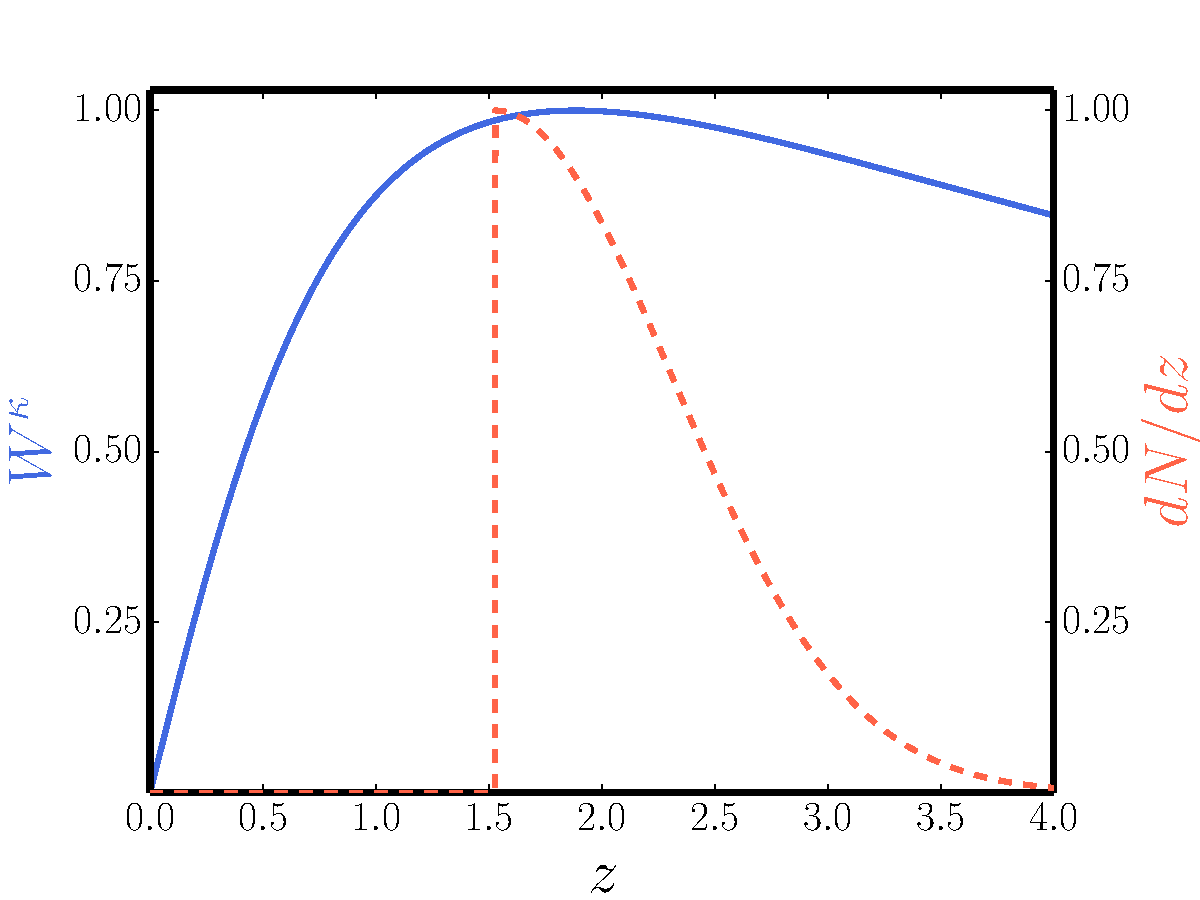
\includegraphics[width=0.7\textwidth]{Chapter3/Images/f1}
\caption{Estimated redshift distribution of the full sample of H-ATLAS galaxies (dashed red line) compared with the \gls{CMB} lensing kernel $W^{\kappa}$ (blue solid line). Both the kernels are normalized to a unit maximum. \label{fig:kernels_norm}}
\end{figure}

%%%%%%%%%%%%%
%%      THEORY            %%
%%%%%%%%%%%%%

\section{Theory and expectations}
\label{sec:theory_xc1}
\subsection{Signal modeling}
We outlined the main features of \gls{CMB} lensing in previous Chapters. Here we briefly recall the quantities which are of relevance for this one.
The effect of gravitational lensing on \gls{CMB} photons can be described as a remapping of the unlensed temperature anisotropies $\Theta(\nver)$ by a two-dimensional vector field in the sky, namely the deflection field $\bm{d}(\nver)$ \citep{Lewis2006}:\footnote{To avoid confusion with $\alpha$, the logarithmic slope of the cumulative number counts of galaxies introduced in Ch.~\eqref{sec:lsslens}, we denote the deflection angle with the letter $\bm{d}(\nver)$.}
\begin{equation}
\begin{split}
\tilde{\Theta}(\hat{\mathbf{n}}) &= \Theta(\nver + \bm{d}(\nver)) \\
&= \Theta(\nver + \nabla\phi(\nver)) \\
&= \Theta(\nver) + \nabla^i \phi(\nver) \nabla_i \Theta(\nver) + \mathcal{O}(\phi^2),
\end{split}
\end{equation}
where $\tilde{\Theta}(\hat{\mathbf{n}})$ are the lensed temperature anisotropies and $\phi(\nver)$ is the \gls{CMB} lensing potential:
\begin{equation}
\phi(\nver) = -2 \int_0^{z_*} \frac{c\,dz}{H(z)}\frac{\chi_* - \chi(z)}{\chi_*\chi(z)}\Phi(\chi(z)\nver,z).
\end{equation}
In this equation, $\chi(z)$ is the comoving distance to redshift $z$, $\chi_*$ is the comoving distance to the last-scattering surface at $z_*\simeq 1090$, $H(z)$ is the Hubble factor at redshift $z$, $c$ is the speed of light, and $\Phi(\chi(z)\nver,z)$ is the three-dimensional gravitational potential at a point on the photon path given by $\chi(z)\nver$. Note that the deflection angle is given by $\bm{d}(\nver) = \nabla\phi(\nver)$, where $\nabla$ is the the two-dimensional gradient on the sphere. Because the lensing potential is an integrated measure of the projected gravitational potential, taking the two-dimensional Laplacian of the lensing potential we can define the lensing convergence $\kappa(\nver) = -\frac{1}{2}\nabla^2\phi(\nver)$, which depends on the projected matter overdensity $\delta$ \citep{Bartelmann2001}:
\begin{equation}
\kappa(\nver) = \int_0^{z_*} dz\, W^{\kappa}(z)\delta(\chi(z)\nver,z).
\label{eqn:wkappa}
\end{equation}
The lensing kernel $W^{\kappa}$ is
%
\begin{equation}
W^{\kappa}(z) = \frac{3\Omega_{\rm m}}{2c}\frac{H_0^2}{H(z)}(1+z)\chi(z)\frac{\chi_*-\chi(z)}{\chi_*},
\end{equation}
%
where $\Omega_{\rm m}$ and $H_0$ are the present-day values of the Hubble and matter density parameters, respectively.

The galaxy overdensity $g(\nver)$ in a given direction on the sky is also expressed as a \gls{LOS} integral of the matter overdensity:
\begin{equation}
g(\nver) = \int_0^{z_*} dz\, W^{g}(z)\delta(\chi(z)\nver,z),
\end{equation}
where the kernel is
\begin{equation}
\label{eqn:wgxc1}
\begin{split}
W^{g}(z) &= \frac{b(z)\frac{dN}{dz}}{\Bigl(\int dz'\,\frac{dN}{dz'}\Bigr)} + \mu(z)\\
&= \frac{b(z)\frac{dN}{dz}}{\Bigl(\int dz'\,\frac{dN}{dz'}\Bigr)} + \frac{3\Omega_{\rm m}}{2c}\frac{H_0^2}{H(z)}(1+z)\chi(z) \int_z^{z_*}dz'\,\Bigl(1-\frac{\chi(z)}{\chi(z')}\Bigr)(\alpha(z')-1)\frac{dN}{dz'}.
\end{split}
\end{equation}
%
Assuming that the luminous matter traces the peaks of the dark matter distribution, the galaxy overdensity kernel is given by the sum of two terms. The first one is related to the physical clustering of sources and is given by the product of the linear bias\footnote{Throughout the analysis we assume a linear, local, deterministic, redshift- and scale-independent bias factor unless otherwise stated.} $b(z)$ and the \emph{unit-normalized} redshift distribution $dN/dz$;  the second one describes the effect of the \emph{lensing magnification bias} \citep{Ho2008,Xia2009} (see also Ch.~\eqref{sec:lsslens}). We recall that this effect depends on the slope, $\alpha(z)$, of their integral counts ($N(>S) \propto S^{-\alpha}$) below the adopted flux density limit. Given the sharply peaked redshift distribution of our sources (see Fig.~\eqref{fig:kernels_norm}) we can safely assume a redshift- and scale-independent linear bias ($b(z)=\hbox{constant}$). Previous analyses of the clustering properties of submillimeter galaxies \cite{Xia2012,Cai2013} indicate $b\simeq 3$ at the redshifts of interest here, and we adopt this as our reference value.

Recent work by \cite{Gonzalez-Nuevo2014} has shown that the magnification bias by weak lensing is substantial for high-$z$ H-ATLAS sources selected with the same criteria as the present sample (see the Sec \eqref{subsec:herschel}). This is because the source counts are steep, although their slope below the adopted flux density limit ($S_{250\mu\rm m}=35\,$mJy) is uncertain. The data \citep{Bethermin2012} indicate, at this limit, $\alpha \simeq 2$ while for the high-$z$ galaxy subsample considered in this work we find $\alpha \simeq 3$, see Fig.~\eqref{fig:s250}. In the following we adopt the latter as our fiducial value. The effect of different choices for this parameter value is examined in Sec~\eqref{sec:discussionxc1}.
%
\begin{figure} %2
\centering % \begin{center}/\end{center} takes some additional vertical space
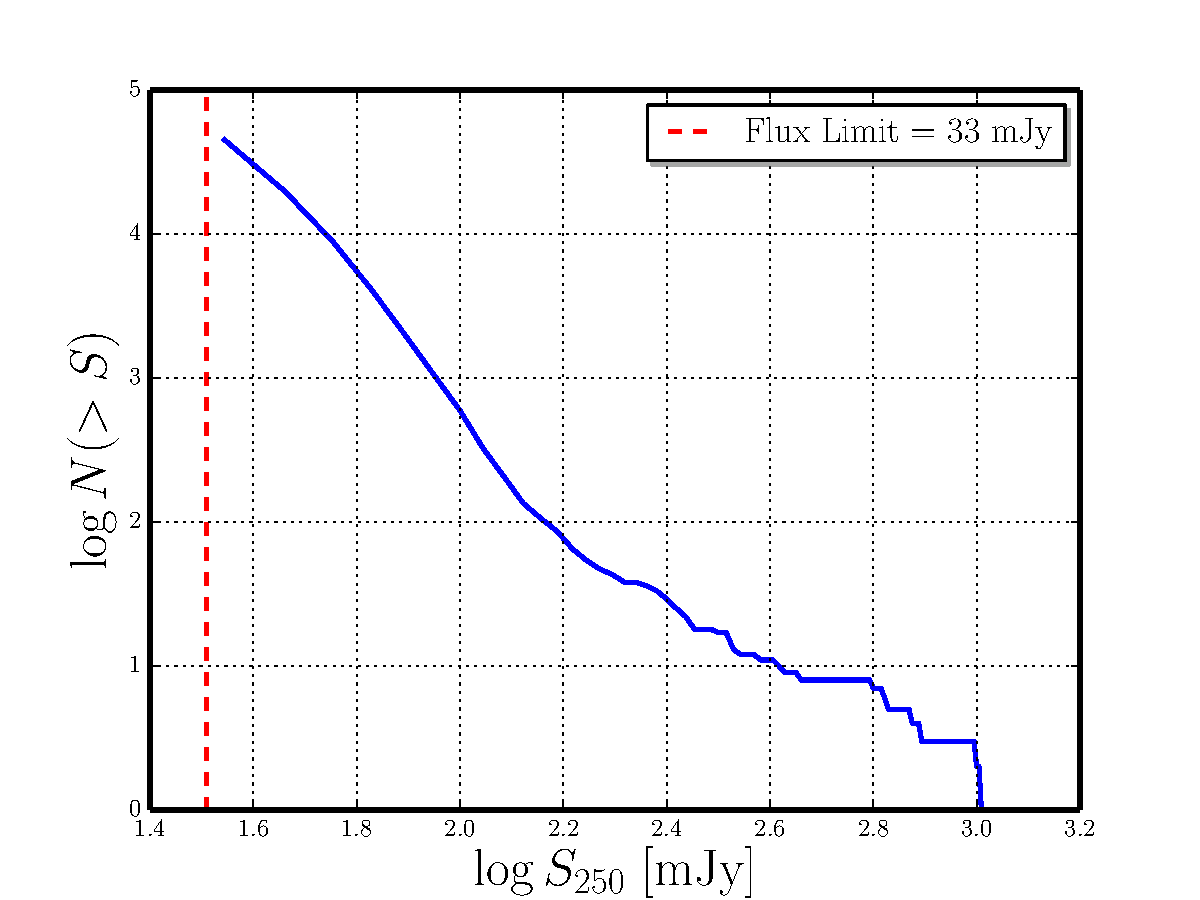
\includegraphics[width=0.6\textwidth]{Chapter3/Images/herschel_counts_250}
\caption{The cumulative number counts of galaxies as function of the flux at 250 $\mu$m, $S_{250 \mu m}$, where the main selection is operated. \label{fig:s250}}
\end{figure}
%
Because the relevant angular scales are much smaller than 1 radian (multipoles $\ell \gtrsim 100$), the theoretical angular cross-correlation can be computed using the Limber approximation \citep{Limber1953a} as
%
\begin{equation}
C_{\ell}^{\kappa g} = \int_0^{z_*} \frac{dz}{c}\frac{H(z)}{\chi^2(z)}W^{\kappa}(z)W^{g}(z)P_{\delta\delta}\Bigl(k=\frac{\ell}{\chi(z)},z\Bigr),
\label{eqn:kg}
\end{equation}
%
where $P_{\delta\delta}(k,z)$ is the matter power spectrum, which we computed using the \texttt{CAMB}\footnote{available at \url{http://camb.info}} code \citep{Lewis2000a}. The nonlinear evolution of the matter power spectrum was taken into account using the \texttt{HALOFIT} prescription \citep{Smith2003,Takahashi2012}. A more extended discussion on the effect of the nonlinear evolution in \gls{CMB} lensing maps based on N-body simulations is carried out by \cite{Antolini2014}. The \gls{CMB} convergence, $W^{\kappa}(z)$, and the galaxy redshift distribution $dN/dz$ of the sample analyzed in this chapter (see Sec~\eqref{subsec:herschel}) are shown in Fig. \eqref{fig:kernels_norm}.

Again under the Limber approximation, the \gls{CMB} convergence, $C_{\ell}^{\kappa\kappa}$, and the galaxy, $C_{\ell}^{gg}$, autospectra can be evaluated as
\begin{equation}
\begin{split}
C_{\ell}^{\kappa\kappa} &= \int_0^{z_*} \frac{dz}{c}\frac{H(z)}{\chi^2(z)}\Bigl[W^{\kappa}(z)\Bigr]^2P_{\delta\delta}\Bigl(k=\frac{\ell}{\chi(z)},z\Bigr); \\
C_{\ell}^{gg} &= \int_0^{z_*} \frac{dz}{c}\frac{H(z)}{\chi^2(z)}\Bigl[W^{g}(z)\Bigr]^2P_{\delta\delta}\Bigl(k=\frac{\ell}{\chi(z)},z\Bigr).
\end{split}
\label{eqn:kkgg}
\end{equation}
%
\subsection{Expected S/N}
Plugging in the specifics of the H-ATLAS survey (see Ch.~\eqref{subsec:herschel} and~\eqref{sec:HSO}), the mean redshift probed by the cross-correlation between \gls{CMB} lensing and our sample is
\begin{equation}\label{eqn:meanz}
\langle z \rangle = \frac{\int_0^{z_*} \frac{dz}{c} z\frac{H(z)}{\chi^2(z)}W^{\kappa}(z)W^{g}(z)P_{\delta\delta}\Bigl(k=\frac{\ell}{\chi(z)},z\Bigr)}{\int_0^{z_*} \frac{dz}{c}\frac{H(z)}{\chi^2(z)}W^{\kappa}(z)W^{g}(z)P_{\delta\delta}\Bigl(k=\frac{\ell}{\chi(z)},z\Bigr)} \simeq 2.
\end{equation}
%
The expected S/N of the convergence-density correlation can be predicted by assuming that both the galaxy {overdensity} and the lensing fields behave as Gaussian random fields, so that the variance of $C_{\ell}^{\kappa g}$ is (see Eq.~\eqref{eq:thvar})
\begin{equation}
\label{eqn:delta_kgxc1}
\bigl(\Delta C_{\ell}^{\kappa g}\bigr)^2 = \frac{1}{(2\ell+1)f_{\rm{sky}}} \bigl[(C_{\ell}^{\kappa g})^2 + (C_{\ell}^{\kappa\kappa}+N_{\ell}^{\kappa\kappa})(C_{\ell}^{gg}+N_{\ell}^{gg})\bigr],
\end{equation}
where $f_{\rm{sky}}$ is the sky fraction covered by both the galaxy and the lensing surveys, $N_{\ell}^{\kappa\kappa}$ is the noise of the lensing field, and $N_{\ell}^{gg}=1/\bar{n}$ is the shot noise associated with the galaxy field. Because our calculations are done in terms of the density contrast, the shot noise is inversely proportional to the mean number of sources per steradian, $\bar{n}$. The signal to noise ratio at multipole $\ell$ is then
\begin{equation}
\label{eqn:s_to_n_mult}
\Bigl( \frac{S}{N} \Bigr)^2_{\ell} = \frac{\bigl(C_{\ell}^{\kappa g}\bigr)^2}{\bigl(\Delta C_{\ell}^{\kappa g}\bigr)^2} = \frac{(2\ell+1)f_{\rm{sky}}\bigl(C_{\ell}^{\kappa g}\bigr)^2 }{\bigl[(C_{\ell}^{\kappa g})^2 + (C_{\ell}^{\kappa\kappa}+N_{\ell}^{\kappa\kappa})(C_{\ell}^{gg}+N_{\ell}^{gg})\bigr]},
\end{equation}
and the cumulative S/N for multipoles up to $\ell_{\rm max}$ is
\begin{equation}
\label{eqn:s_to_n_cum}
\Bigl( \frac{S}{N} \Bigr)(<\ell_{\rm max}) = \sqrt{\sum_{\ell'=\ell_{\rm min}}^{\ell_{\rm max}} \Bigl( \frac{S}{N} \Bigr)^2_{\ell'}}.
\end{equation}
%
In Fig. \eqref{fig:s_to_n_hatlas} we show both the S/N per multipole and the cumulative one computed using the specifications for the \textit{Planck} lensing noise (see Sec ~\eqref{subsec:planckxc1}) and the mean surface density of our source sample. It must be noted that, because of the limited area covered by the H-ATLAS survey (and split into 5 fields), the cross-correlation is only meaningful on scales below a few degrees. We have therefore limited our analysis to $\ell \ge \ell_{\rm min} = 100$. This restriction prevents us from exploiting the peak at $\ell \sim 100$ of the signal to noise per multipole. The cumulative S/N saturates at $\ell \sim 1000$. If $b=3$ and $\alpha=3$ we expect $S/N \simeq 6$.

\begin{figure} %2
\centering % \begin{center}/\end{center} takes some additional vertical space
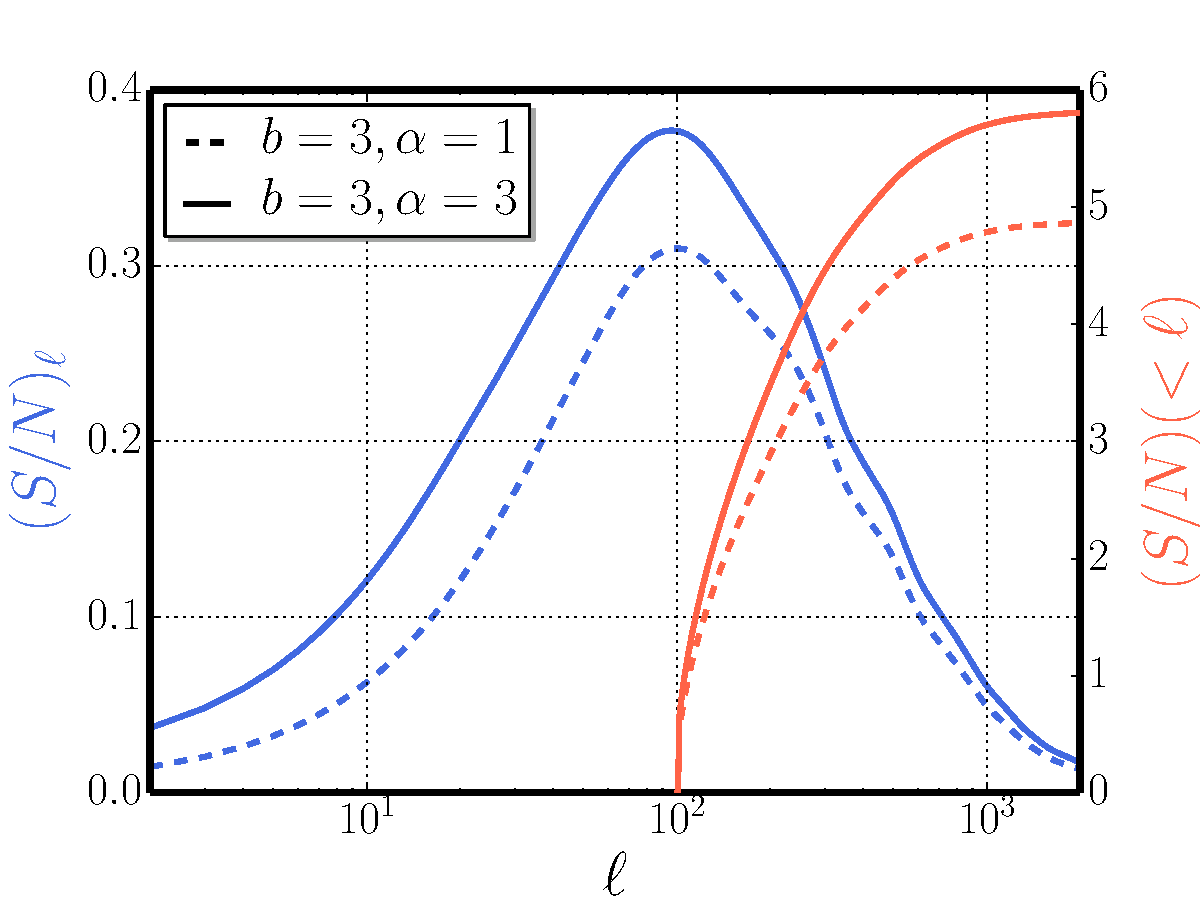
\includegraphics[width=0.7\textwidth]{Chapter3/Images/f2}
\caption{S/N per multipole (blue lines; left axis) and cumulative S/N (red lines; right axis) evaluated from $\ell_{\rm min}=100$ for fiducial models with $b=3$ and $\alpha=1$ (no magnification, dashed lines) and $\alpha=3$ (solid lines). \label{fig:s_to_n_hatlas}}
\end{figure}

%%%%%%%%%%%%%
%%          DATA            %%
%%%%%%%%%%%%%

\section{Data}
\label{sec:dataxc1}
Both the \textit{Planck} \gls{CMB} lensing and \textit{Herschel} submillimeter galaxies datasets used in this analysis have been previously introduced in Ch.~\eqref{sec:datasets}; we recall here the main aspects of interest for this Chapter.

\subsection{\emph{Planck} data}
\label{subsec:planckxc1}
We used the publicly released \emph{Planck} \gls{CMB} lensing potential map derived from the first 15.5 months of observations \citep{Ade2014c}. The released map is based on a minimum variance combination of the 143 and 217 GHz temperature anisotropy maps only, because adding the 100 GHz map yields a negligible improvement \citep{Ade2014c}.\footnote{We recall that the angular resolution and the noise level  of the 100, 143 and 217 GHz frequency channels are $10'$, $7'$, $5'$ and 105, 45, 60 $\mu$K\,arcmin respectively.} The maps are in the HEALPix format with a resolution parameter of $N_{\rm side} = 2048$, corresponding to 50, 331, and 648 pixels over the sky, with a pixel size of $\sim 1.7'$.

\begin{figure} %  3
\centering % \begin{center}/\end{center} takes some additional vertical space
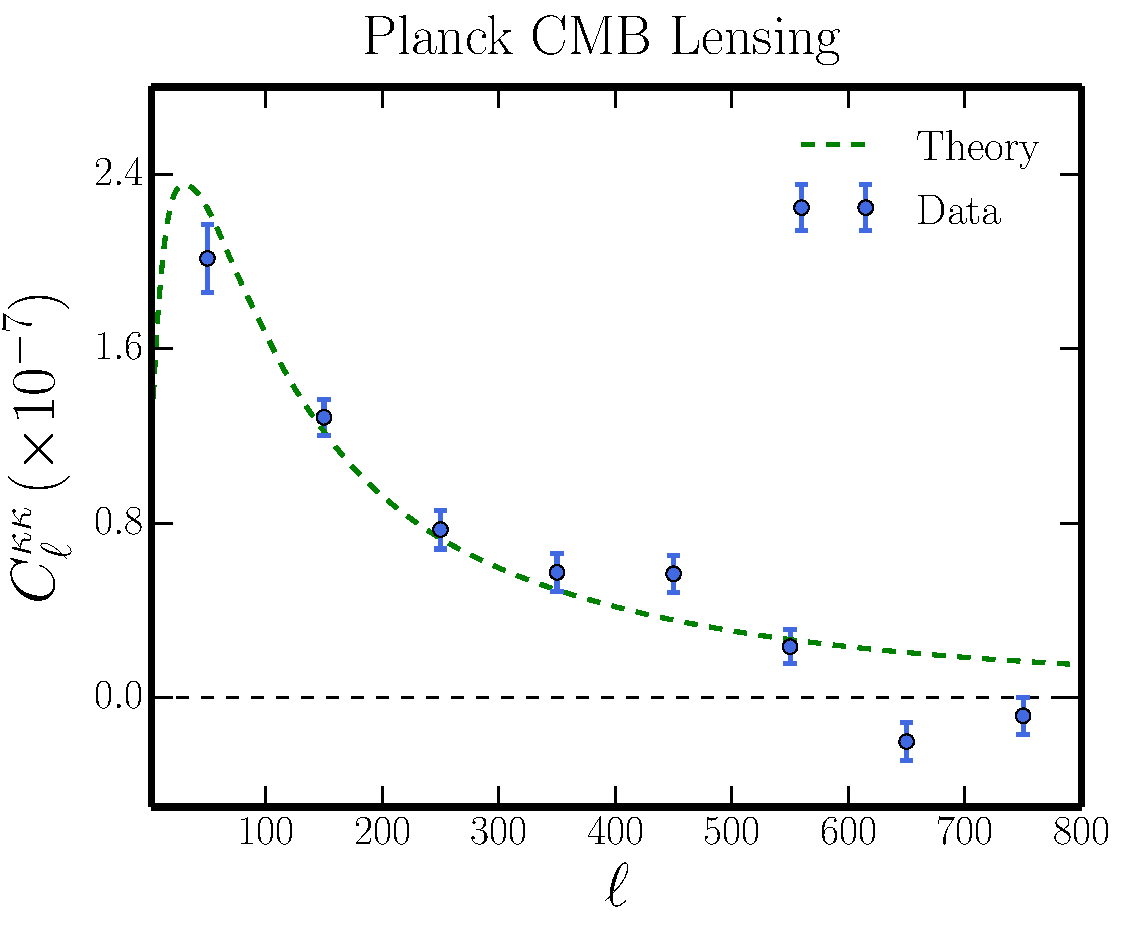
\includegraphics[width=0.7\textwidth]{Chapter3/Images/f3}
\caption{\gls{CMB} convergence autopower spectrum as reconstructed from \emph{Planck} data (blue points) on a portion of the sky with $f_{\rm{sky}} \simeq 0.6$ compared with the theoretical prediction for our background cosmology (dashed green line).
 \label{fig:kk_data_planck}}
\end{figure}

The power spectrum of the lensing potential is very red, and this may introduce a bias when we estimate it within multipole bins. To avoid this problem, we decided to convert the lensing potential map, $\phi$, into the convergence map, $\kappa$, which has a much less red power spectrum.
This was done using the relation between the spherical harmonic coefficients of these quantities estimated on the full sky \citep{Hu2000}
\begin{equation}
\kappa_{\ell m} = -\frac{\ell(\ell+1)}{2}\phi_{\ell m} \ .
\end{equation}
The convergence spherical harmonic coefficients were transformed to a map with resolution parameter $N_{\rm side}=512$ corresponding to a pixel size of $\sim 7'$. This resolution is sufficient for our analysis because the data noise level enables us to detect cross-correlations between the convergence and the galaxy density field only for angular scales larger than $\sim 20'$ ($\ell \lesssim 540$).

The convergence autopower spectrum recovered on approximately $60\%$ of the sky using a modified version of the mask provided by the \textit{Planck} collaboration is shown in Fig.~\eqref{fig:kk_data_planck}. The auto-power spectrum has been corrected for the lensing reconstruction noise power spectrum  $N_{\ell}^{\kappa\kappa}$ which was estimated from the set of 100 simulated lensing maps\footnote{\url{http://irsa.ipac.caltech.edu/data/Planck/release_1/ancillary-data/HFI_Products.html}} recently released by the \emph{Planck} team that account for the inhomogeneous noise level. The noise power spectrum was computed by averaging the spectra of the difference maps between the reconstructed and the input lensing map over 100 realizations. The errors on band powers were calculated as the diagonal part of the covariance matrix built from the simulation, as described in Sec.~\eqref{sec:estimatorxc1}. The raw auto-power spectrum is not corrected for the bias induced by non-Gaussianity of unresolved point sources and for pseudo-$C_{\ell}$ leakage effects from masking (we just correct for N0 and N1 bias term adopting the formalism of \cite{Ade2014c}). These terms may cause some discrepancy of the power spectrum at high multipoles. Nevertheless, in the range of multipoles relevant for our analysis the power spectrum agrees pretty well with the theoretical one, and proper estimation of the convergence power spectrum is outside the scope of this thesis.

\subsection{\textit{Herschel} fields}
\label{subsec:herschel}

We exploited the data collected by the \textit{Herschel} Space Observatory \citep{Pilbratt2010} in the context of the \textit{Herschel} Astrophysical Terahertz Large Area Survey (H-ATLAS) \citep{Eales2010a}, an open-time key program that has surveyed about $600$ deg$^2$ with the Photodetector Array Camera and Spectrometer (PACS) \citep{Poglitsch2010} and the Spectral and Photometric Imaging Receiver (SPIRE) \citep{Griffin2010} in five bands, from $100$ to $500\,\mu$m. 

The surveyed area is divided into five fields: three equatorial fields centered on 9hr, 12hr, and 14.5hr (GAMA fields, G09, G12, and G15) covering, altogether, $161\,\hbox{deg}^2$; the NGP block; and the SGP block consisting of two concatenated rectangular regions. The footprint of the survey is shown in the right panel of Fig.~\eqref{fig:masks}.

The H-ATLAS galaxies have a broad redshift distribution extending from $z=0$ to $z\simeq 5$ \citep{Pearson2013}. The $z \lesssim 1$ population is mostly made of ``normal'' late-type and star-burst galaxies with low to moderate star formation rates  \citep[SFRs;][]{Dunne2011,Guo2011} while the high-$z$ galaxies are forming stars at high rates ($\hbox{SFR}\gtrsim \hbox{few hundred}\,M_{\odot}\,\hbox{yr}^{-1}$) and are much more strongly clustered \citep{Maddox2010,Xia2012}, implying that they are tracers of large-scale overdensities. Their properties are consistent with them being the progenitors of local massive elliptical galaxies \citep{Lapi2011}. We aim to correlate high-$z$ H-ATLAS galaxies with the \textit{Planck} \gls{CMB} lensing map.

To select the high-$z$ population, we adopted the criteria developed by \cite{Gonzalez-Nuevo2012}: 
\begin{enumerate}
\item{$S_{250\,\mu\rm m}>35$ mJy;}
\item{$S_{350\,\mu\rm m}/S_{250\,\mu\rm m}>0.6$ and $S_{500\,\mu\rm m}/S_{350\,\mu\rm m}>0.4$;} 
\item{$3\,\sigma$ detection at $350\,\mu$m;} 
\item{photometric redshift $z_{\rm phot}>1.5$, estimated following \cite{Lapi2011} and \cite{Gonzalez-Nuevo2012}.}
\end{enumerate}

Our final sample comprises a total of 99,823 sources, of which $9,099$ are in G09, $8,751$ in G12, $9,279$ in G15, $28,245$ in NGP and $44,449$ in SGP. The specifics of each patch are summarized in Table~\eqref{herschel_patches_xc1}. The redshift distribution of the population is needed in order to predict the amplitude of the cross-correlation. Estimating the uncertainties in the redshift distribution due to photometric redshift errors is not a trivial task. 

As stated in \cite{Gonzalez-Nuevo2012} there is no indication that photometric redshifts are systematically under- or overestimated when the spectral energy distribution of SMM J2135-0102 is used as a template. The median value of $ \Delta z/(1 + z) \equiv (z_{\rm phot} -  z_{\rm spec})/(1 + z_{\rm spec})$ is -0.002 with a dispersion of 0.115. This dispersion corresponds to an rms error on $z$ of $\sigma_{\langle z \rangle}=  0.345$ at the mean redshift $\langle z \rangle\simeq 2$, given by Eq.~(\eqref{eqn:meanz}). To get a rough indication of how many sources were scattered above and below the redshift threshold ($z=1.5)$ by measurement errors we have convolved a gaussian fit to the redshift distribution of sources selected with the first 3 criteria [(1) to (3)] with a gaussian error distribution having zero mean and dispersion $\sigma_{\langle z \rangle}$. The convolved redshift distribution was cut at $z = 1.5$, and the portion at higher $z$ was fitted with a half-normal distribution normalized to unity:
%
\begin{equation}
\frac{dN}{dz} = \frac{\sqrt{2}}{\sigma\sqrt{\pi}}\exp{\Bigl( -\frac{(z-\mu)^2}{2\sigma^2}\Bigr)}.
\end{equation}
%
The redshift distributions of the galaxies before and after the convolution are shown in Fig.~\eqref{fig:dndzxc1}.

We built an overdensity map at a resolution $N_{\rm side}=512$ defined by
%
\begin{equation}
\label{eqn:counttodensity}
g(\nver) = \frac{n(\nver)-\bar{n}}{\bar{n}},
\end{equation}
%
where $n(\nver)$ is the number of objects in a given pixel, and $\bar{n}$ is the mean number of objects per pixel. The \gls{CMB} convergence and galaxy overdensity maps in the different patches are shown in Fig.~\eqref{fig:patches}. We filtered out from these fields multipoles $\ell \gtrsim 400$ where $(S/N)_{\ell}\lesssim 0.3$.

\begin{figure} %4
\centering % \begin{center}/\end{center} takes some additional vertical space
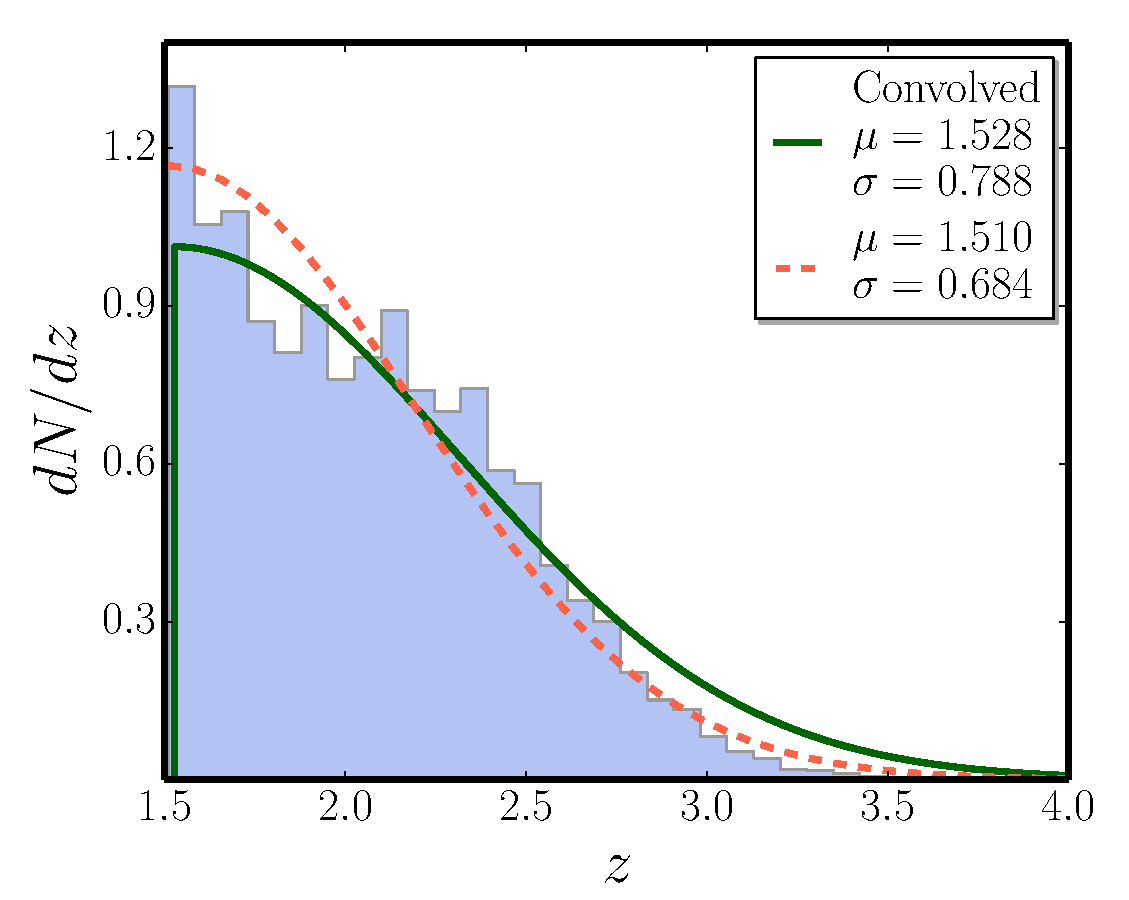
\includegraphics[width=0.6\textwidth]{Chapter3/Images/f4}
\caption{Redshift distribution of H-ATLAS galaxies for the combined set of patches used in the analysis. The (blue) histogram  is the empirical redshift distributions, the dashed (orange) line is the half-normal fit to $dN/dz$ as described in text, while the solid (green) line represents the convolved $dN/dz$ that takes into account errors on photo-z estimation and is used as the fiducial distribution in our analysis. The values of the parameters $\mu$ and $\sigma$ given in the box are the best-fit values and are used in the analytic expression for $dN/dz$ adopted in calculations. \label{fig:dndzxc1}}
\end{figure}

%\begin{deluxetable}{ccccc}
%\tabletypesize{}
%%\rotate
%\tablecaption{H-ATLAS Patches Data\label{herschel_patches}}
%\tablewidth{0pt}
%\tablehead{
%{Patch} & {$N_{\rm obj}$} & {$f_{\rm{sky}}$} & {$\bar{n}\,[\hbox{gal}\,\hbox{pix}^{-1}]$} & {$\bar{n}\,[\hbox{gal}\,\hbox{sr}^{-1}]$}
%}
%\startdata
%ALL   &   99823 &   0.014   &    2.30    &    $5.76\times 10^5$ \\
%NGP  &   28245 &   0.004   &    2.25    &    $5.64\times 10^5$ \\
%SGP  &   44449 &   0.006   &    2.38    &    $5.95\times 10^5$ \\
%G09   &   9099   &   0.001   &    2.28    &    $5.71\times 10^5$ \\
%G12   &   8751   &   0.001   &    2.13    &    $5.35\times 10^5$ \\
%G15   &   9279   &   0.001   &    2.27    &    $5.68\times 10^5$ \\
%\enddata
%\tablenotetext{a}{ALL is  the combination of all the patches together.}
%\end{deluxetable}

\begin{table}[t]
\centering
\caption{H-ATLAS Patches Data\label{herschel_patches_xc1}}
\begin{threeparttable}
\begin{tabular}{ccccc}
\toprule
\midrule
Patch & $N_{\rm obj}$ & $f_{\rm{sky}}$ & $\bar{n}\,[\hbox{gal}\,\hbox{pix}^{-1}]$ & $\bar{n}\,[\hbox{gal}\,\hbox{sr}^{-1}]$\\
\midrule
ALL\tnote{a}  &   99823 &   0.014   &    2.30    &    $5.76\times 10^5$ \\
NGP  &   28245 &   0.004   &    2.25    &    $5.64\times 10^5$ \\
SGP  &   44449 &   0.006   &    2.38    &    $5.95\times 10^5$ \\
G09   &   9099   &   0.001   &    2.28    &    $5.71\times 10^5$ \\
G12   &   8751   &   0.001   &    2.13    &    $5.35\times 10^5$ \\
G15   &   9279   &   0.001   &    2.27    &    $5.68\times 10^5$ \\
\bottomrule
\end{tabular}
\begin{tablenotes}
\item[a] ALL is the combination of all fields together.
\end{tablenotes}
\end{threeparttable}
\end{table}

\begin{figure*}[t] %5
\centering % \begin{center}/\end{center} takes some additional vertical space
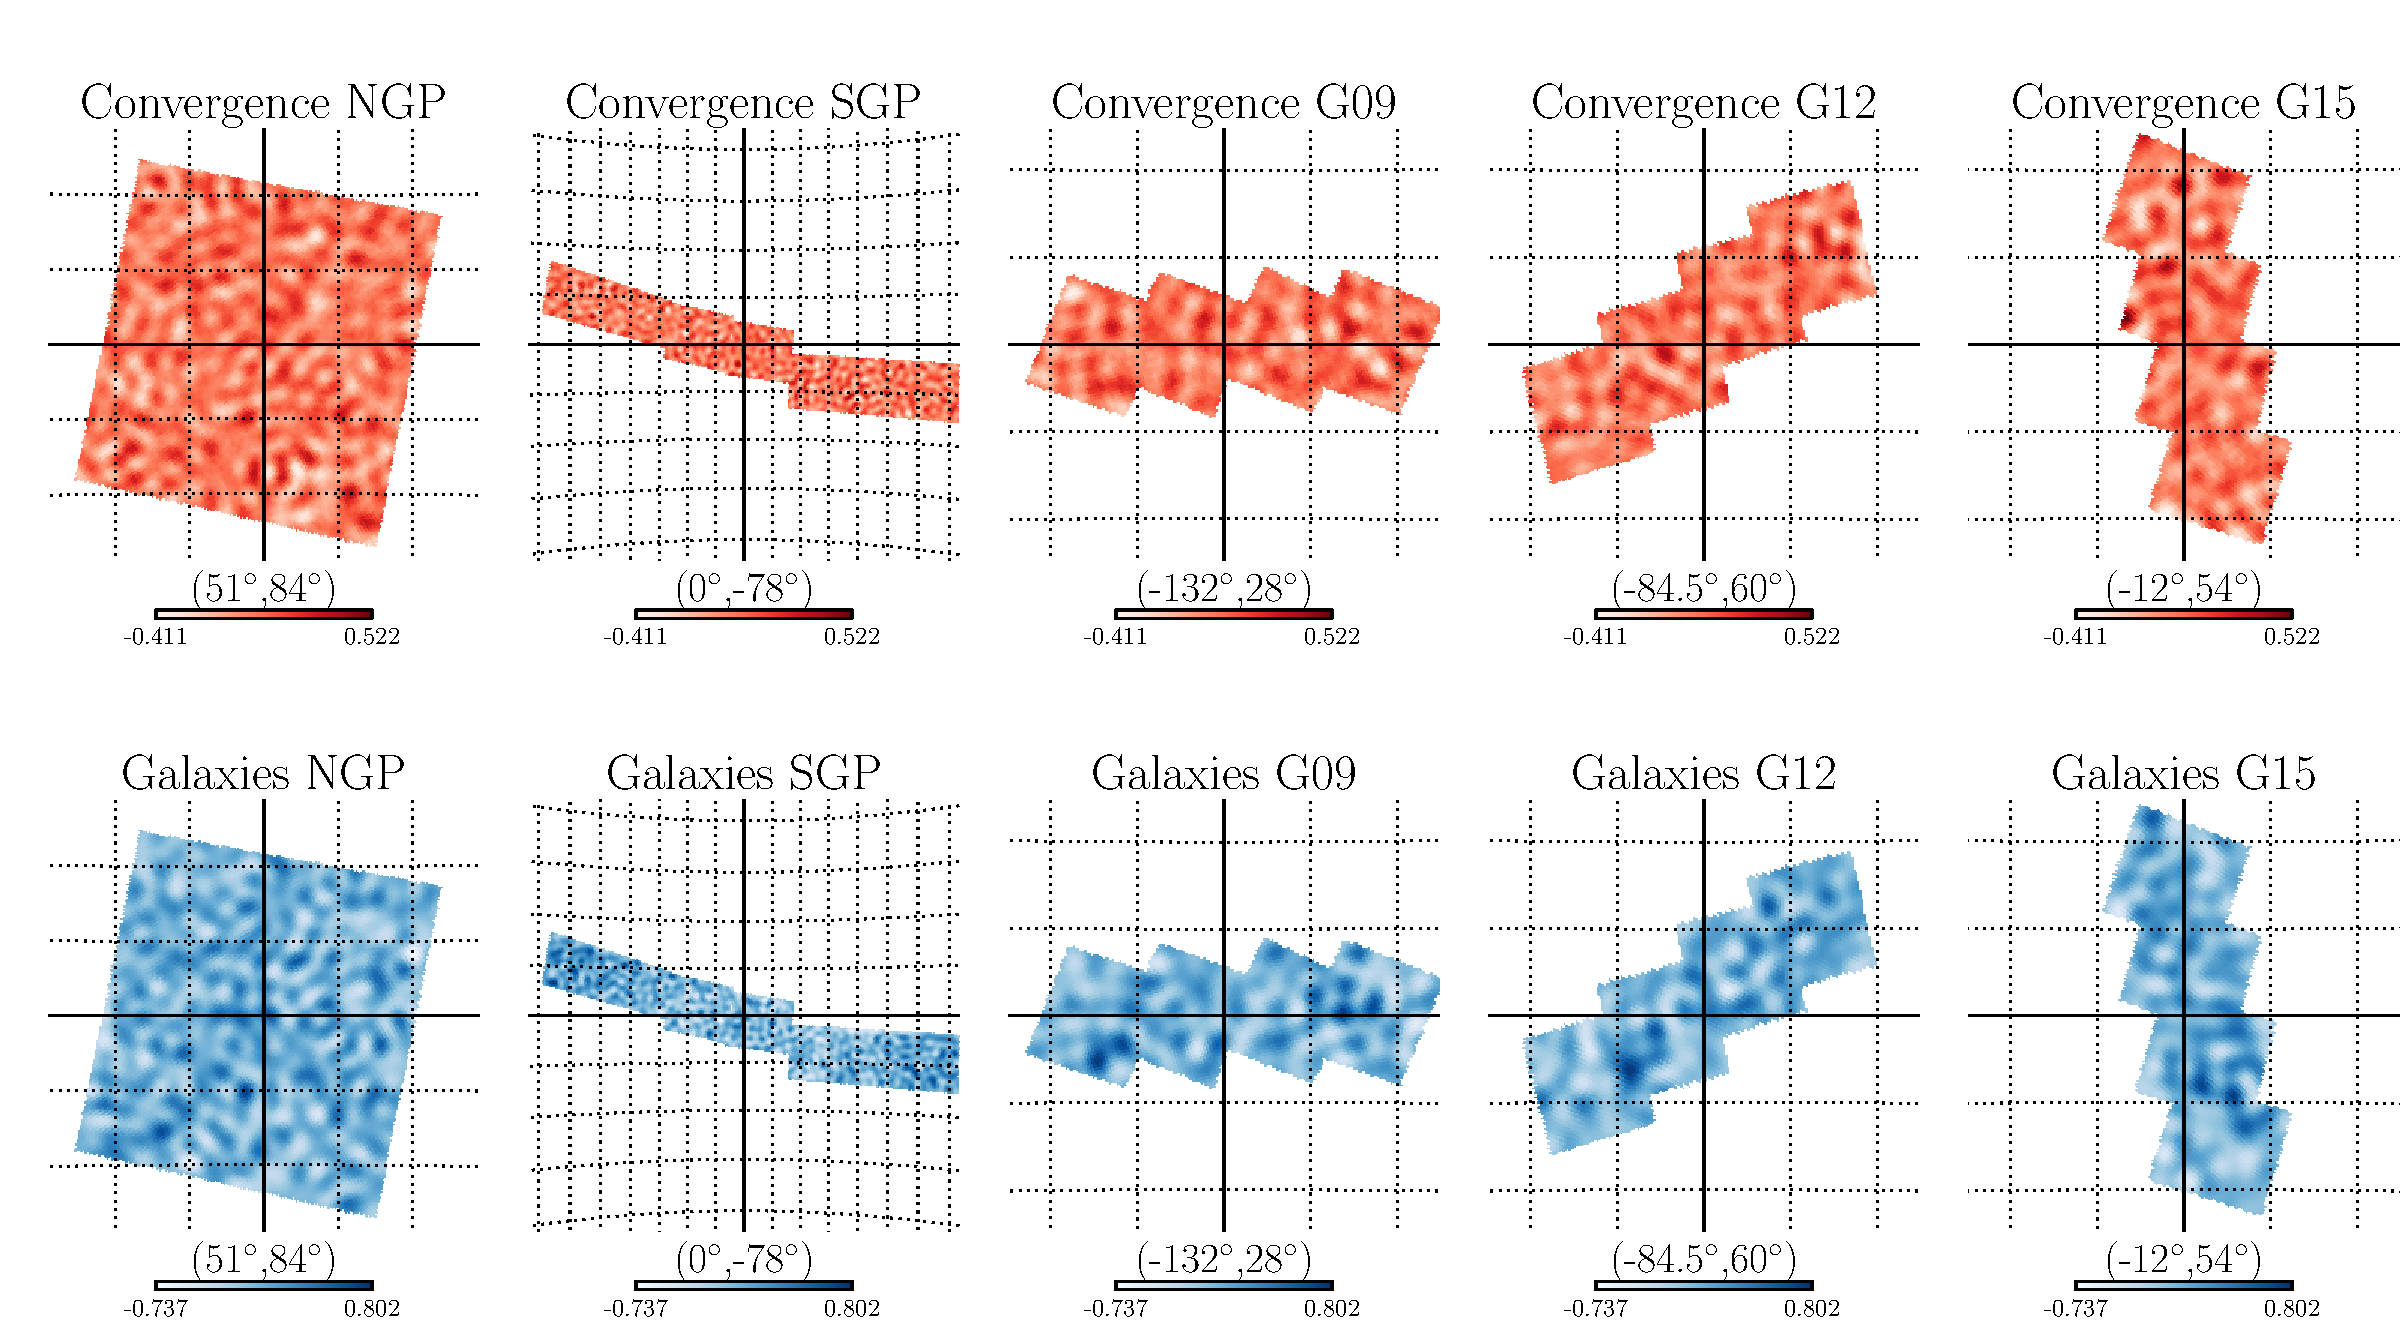
\includegraphics[width=\textwidth]{Chapter3/Images/f5}
\caption{Convergence maps (upper row) and galaxy overdensity maps (lower row) in the H-ATLAS fields: multipoles $\ell > 400$ for which $(S/N)_{\ell} \lesssim 0.3$ have been filtered out. Galactic longitude and latitude $(l,b)$ of patch centers are provided in brackets. The grid overlay has spacing of $3^\circ$ in each box. \label{fig:patches}}
\end{figure*}

%%%%%%%%%%%%%
%%  XC ALGORITHM  %%
%%%%%%%%%%%%%

\section{The Cross-Correlation Algorithm}
\label{sec:estimatorxc1}

\subsection{Estimator}

We computed the angular power spectra within the regions covered by the H-ATLAS survey using a \gls{PCL} estimator based on the \texttt{MASTER} algorithm \citep{Hivon2001a}.\footnote{These regions are inside the area used in the estimation of the \gls{CMB} lensing map.}  In Ch.~\eqref{sec:ps_est} we have extensively discussed \gls{PCL} methods, here we just recall the main aspects and contextualize to the case of the \gls{CMB} lensing-galaxy cross-correlation. For a survey that covers only a fraction of the sky, different modes of the true cross-power spectrum $C^{\kappa g}_{\ell}$ are coupled \citep{Hauser1973}. The coupling can be described by the mode-mode coupling matrix $M_{\ell\ell'}$ which relates the pseudo-cross-spectrum $\tilde{C}^{\kappa g}_{\ell}$ measured from the data
%
\begin{equation}
\tilde{C}^{\kappa g}_{\ell} = \frac{1}{2\ell+1}\sum_{m=-\ell}^{\ell} \tilde{\kappa}_{\ell m}\tilde{g}^*_{\ell m}.
\end{equation}
%
to the true spectrum
%
\begin{equation}
\label{eqn:coupling}
\tilde{C}_{\ell}^{\kappa g} = \sum_{\ell'} M_{\ell\ell'}C_{\ell'}^{\kappa g}.
\end{equation}
%
However, we cannot directly invert Eq.~\eqref{eqn:coupling} to get the true power spectrum, because for surveys covering only a small fraction of the sky, the coupling matrix $M_{\ell\ell'}$ becomes singular.  To reduce the correlations of the $C_{\ell}$'s it is necessary to bin the power spectrum in $\ell$. We used eight linearly spaced bins of width $\Delta\ell = 100$ in the range $0 \le \ell \le 800$.

Then, the estimator of the true band powers $\hat{C}^{\kappa g}_{L}$ (hereafter $C^{\kappa g}_{L}$ denotes the binned power spectrum and  $L$ identifies the bin) is given by
%
\begin{equation}
\label{eqn:master_kgxc1}
\hat{C}^{\kappa g}_{L} = \sum_{L' \ell}K^{-1}_{LL'}P_{L'\ell}\tilde{C}^{\kappa g}_{\ell},
\end{equation}
%
where
%
\begin{equation}
K_{LL'} = \sum_{\ell\ell'} P_{L\ell}M_{\ell\ell'}p^2_{\ell'}Q_{\ell' L'}.
\end{equation}
%
Here $P_{L\ell}$ is the binning operator; $Q_{\ell L}$ and $p^2_{\ell'}$ are, respectively, the reciprocal of the binning operator and  the pixel window function that takes into account the finite pixel size. Because of the small size of the sky area covered by the H-ATLAS survey, the power spectrum for $\ell < 100$ is very poorly estimated, and we did not use it in our analysis. However, to avoid the bias coming from the lowest-order multipoles, the first multipole bin is included in the computation of the power spectrum; that is, the inversion of the binned coupling matrix $K_{LL'}$ is performed including the first bin, and the pseudopower spectrum for the first bin is used in the product of Eq.~\eqref{eqn:master_kgxc1}.

The main assumption in cross-correlation studies is that the noise levels related to the observables being analyzed are uncorrelated, so that we do not need to debias the reconstructed cross-spectrum for any noise term. However, when dealing with autopower spectra, such as $C^{gg}_{\ell}$ and $C^{\kappa\kappa}_{\ell}$, we have to correct the estimator given by Eq.~\eqref{eqn:master_kgxc1} in order to account for the noise:
%
\begin{equation}
\begin{split}
\hat{C}^{gg}_{L} &= \sum_{L'\ell}K^{-1}_{LL'}P_{L'\ell}\Bigl( \tilde{C}^{gg}_{\ell} - \langle \tilde{N}^{gg}_{\ell}\rangle_{\rm{MC}} \Bigr), \\
\hat{C}^{\kappa\kappa}_{L} &= \sum_{L'\ell}K^{-1}_{LL'}P_{L'\ell}\Bigl( \tilde{C}^{\kappa\kappa}_{\ell} - \langle \tilde{N}^{\kappa\kappa}_{\ell}\rangle_{\rm{MC}} \Bigr),
\end{split}
\end{equation}
%
where $\langle \tilde{N}^{gg}_{\ell}\rangle_{\rm{MC}}$ and $\langle \tilde{N}^{\kappa\kappa}_{\ell}\rangle_{\rm{MC}}$ are the average noise pseudospectra estimated from the \gls{MC} simulations.

\subsection{Covariance matrix}\label{sec:covxc1}
The errors on the cross-power spectrum are described by the covariance matrix \citep{Brown2005}
%
\begin{equation}
\label{eqn:analytic_covariance}
 \text{Cov}^{\kappa g}_{LL'} = M_{LL_1}^{-1} P_{L_1\ell}\,\widetilde{\text{Cov}}^{\kappa g}_{\ell\ell'} \, Q_{\ell' L_2} (M_{L'L_2}^{-1})^T,
\end{equation}
%
where $\widetilde{\text{Cov}}^{\kappa g}_{\ell\ell'}$ is the pseudocovariance matrix given by
%
\begin{equation}
\begin{split}
\label{eqn:pcov_kg}
 &\widetilde{\text{Cov}}^{\kappa g}_{\ell\ell'}  =  \frac{1}{2\ell'+1}M_{\ell\ell'}\Bigl[ C_{\ell}^{\kappa g}(b)C_{\ell'}^{\kappa g}(b)+ \\
 & \sqrt{(C_{\ell}^{\kappa\kappa}+N_{\ell}^{\kappa\kappa})(C_{\ell}^{gg}(b) + N_{\ell'}^{gg})(C_{\ell'}^{\kappa\kappa}+N_{\ell'}^{\kappa\kappa})(C_{\ell'}^{gg}(b) + N_{\ell'}^{gg})}\Bigr].
\end{split}
\end{equation}
%
The corresponding covariance matrix of the galaxy autocorrelation is obtained by replacing in Eq.~(\eqref{eqn:analytic_covariance}) the pseudocovariance matrix $\widetilde{\text{Cov}}^{\kappa g}_{\ell\ell'}$ with  $\widetilde{\text{Cov}}^{gg}_{\ell\ell'}$ given by
%
\begin{equation}
\label{eqn:pcov_gg}
 \widetilde{\text{Cov}}^{gg}_{\ell\ell'} = \frac{2}{2\ell'+1}M_{\ell\ell'}\Bigl[(C_{\ell}^{gg}(b) + N_{\ell}^{gg})(C_{\ell'}^{gg}(b) + N_{\ell'}^{gg})\Bigr].
\end{equation}
%
The analytical expressions for the covariance matrices given above were used in the estimation of the galaxy bias and of the amplitude of the cross-correlation, presented in Sec \eqref{sec:constraintsxc1}.

\subsection{Validation}
In order to validate the algorithms used for the computation of the estimators outlined in the previous section and to check that the cross- and autopower spectra estimates are unbiased, we created 500 simulated maps of the \gls{CMB} convergence field and of the galaxy overdensity field with statistical properties consistent with observations.

Using the theoretical spectra obtained with Eqs. \eqref{eqn:kg} and \eqref{eqn:kkgg}, we generated full-sky signal maps, injecting a known degree of correlation, so that the simulated \gls{CMB} convergence and galaxy harmonic modes satisfy both the auto- and the cross-correlations \citep{Kamionkowski1997}:
%
\begin{equation}
\begin{split}
\kappa_{\ell m} &= \zeta_1 \bigl(C_{\ell}^{\kappa\kappa} \bigr)^{1/2};\\
g_{\ell m} &= \zeta_1 \frac{C_{\ell}^{\kappa g}}{\bigl(C_{\ell}^{\kappa\kappa} \bigr)^{1/2}} + \zeta_2 \Biggl[ C_{\ell}^{gg} - \frac{\bigl(C_{\ell}^{\kappa g}\bigr)^2}{C_{\ell}^{\kappa\kappa}} \Biggr]^{1/2}.
\end{split}
\end{equation}
%
For each value of $\ell$ and $m>0$, $\zeta_1$ and $\zeta_2$ are two complex numbers drawn from a Gaussian distribution with unit variance, whereas for $m=0$ they are real and normally distributed.

We also generated 500 noise realizations for both fields. To simulate Gaussian convergence noise maps, we used the convergence noise power spectrum $N^{\kappa\kappa}_{\ell}$ available at the \textit{Planck Legacy Archive}\footnote{\url{http://wiki.cosmos.esa.int/planckpla/index.php/Specially_processed_maps}} (PLA). Although this power spectrum is not sufficiently accurate to estimate the convergence power spectrum, it should be sufficiently good for the cross-correlation analysis, which is not biased by the noise term. For the same reason, it is not crucial for our analysis to use the 100 simulations of the estimated lensing maps available at the PLA.

To take into account noise in the simulated galaxy maps, we proceeded in the following way. For each signal map containing the galaxy overdensity, we generated a set of  simulated galaxy number count maps, where the value in each pixel is drawn from a Poisson distribution with mean
%
\begin{equation}
\lambda(\nver) = \bar{n}(1+g(\nver)),
\end{equation}
%
where $\bar{n}$ is the mean number of sources per pixel in a given H-ATLAS patch and $g(\nver)$ is the corresponding simulated galaxy map containing only signal. The galaxy number counts map $\lambda(\nver)$ was then converted into a galaxy overdensity map using Eq.~\eqref{eqn:counttodensity}, substituting the real number of objects in a given pixel $n(\nver)$ with the simulated one $\lambda(\nver)$. Note that maps obtained in this way already include Poisson noise with variance $N^{gg}_{\ell} = 1/\bar{n}$.

We applied the pipeline described above to our set of simulations in order to recover the input cross- and autopower spectra used to generate such simulations. The extracted $\hat{C}^{\kappa g}_{L}$, $\hat{C}^{gg}_{L}$, and $\hat{C}^{\kappa\kappa}_{L}$  spectra averaged over 500 simulations are reported in Fig.~\eqref{fig:validation}.  The mean band power was computed as
\begin{equation}
\langle \hat{C}^{XY}_{L} \rangle = \frac{1}{\Nsim}\sum_{i=1}^{\Nsim} \hat{C}^{XY,i}_{L},
\end{equation}
where $X,Y = \{\kappa,g\}$, $i$ refers to the $i$-th simulation, and $\Nsim=500$ is the number of simulations. The errors were computed from the covariance matrix as
%
\begin{equation}
\Delta \hat{C}^{XY}_{L} = \Bigl(\frac{\cov^{XY}_{LL}}{\Nsim} \Bigr)^{1/2},
\end{equation}
%
and the covariance matrix $\cov^{XY}_{LL'}$ was evaluated from the simulations as
%
\begin{equation}
\cov^{XY}_{LL'} = \frac{1}{\Nsim-1} \sum_{i=1}^{\Nsim} ( \hat{C}^{XY,i}_{L} - \langle \hat{C}^{XY}_{L}\rangle_{\rm{MC}})( \hat{C}^{XY,i}_{L'} - \langle \hat{C}^{XY}_{L'}\rangle_{\rm{MC}}).
\end{equation}
%
We also show, for comparison, the theoretical error bars obtained from Eq.~(\eqref{eqn:delta_kgxc1}), modified to take into account the binning. They are in generally good agreement with the \gls{MC} error estimates, which, however, are slightly larger (by up to $\sim 25 \%$).

\begin{figure*}
\centering
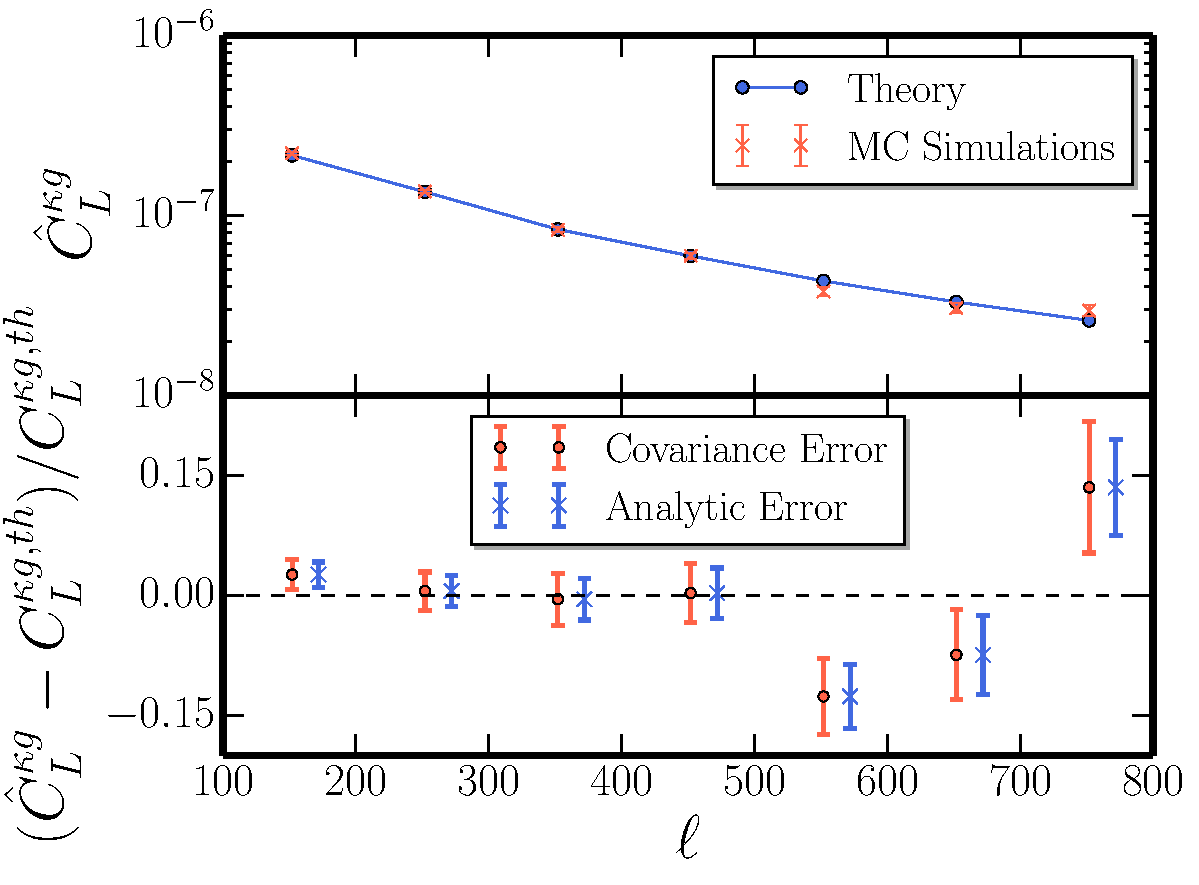
\includegraphics[scale=0.4]{Chapter3/Images/f6}\\
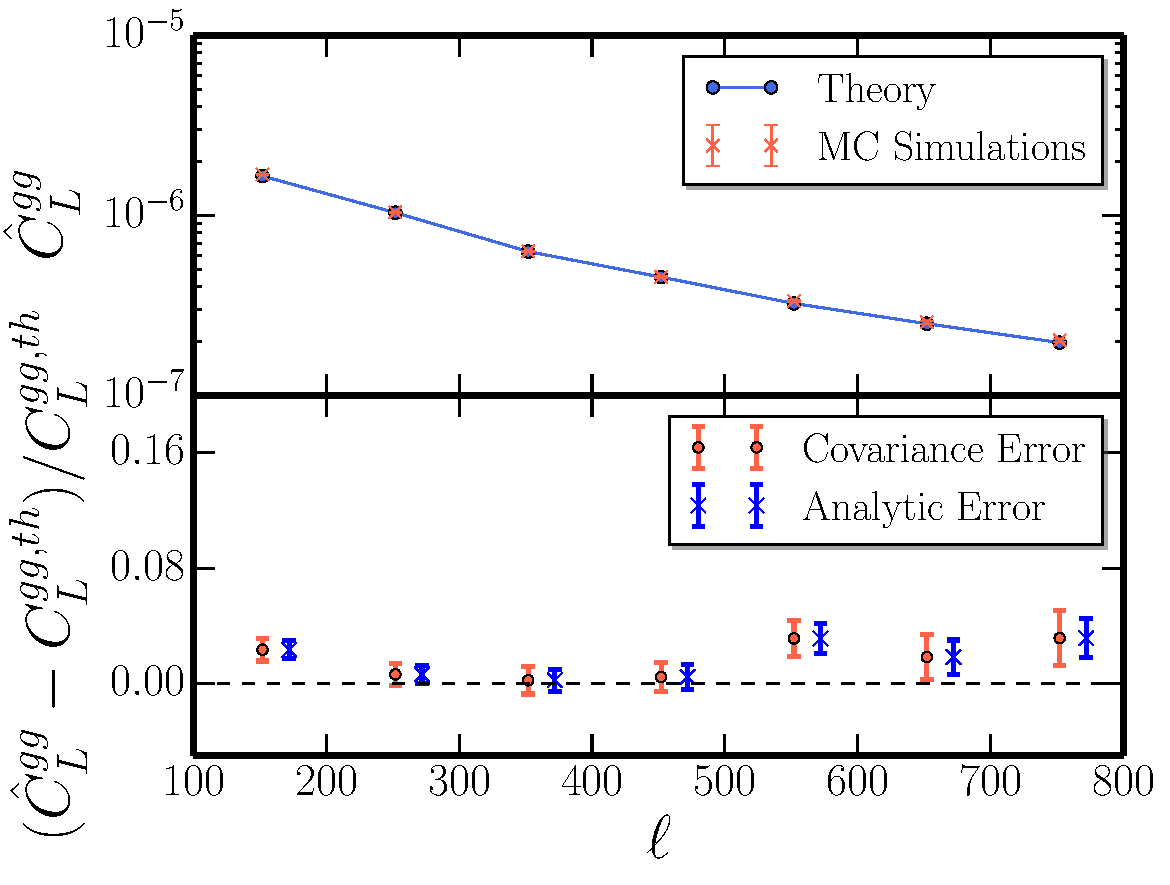
\includegraphics[scale=0.4]{Chapter3/Images/f7}\\
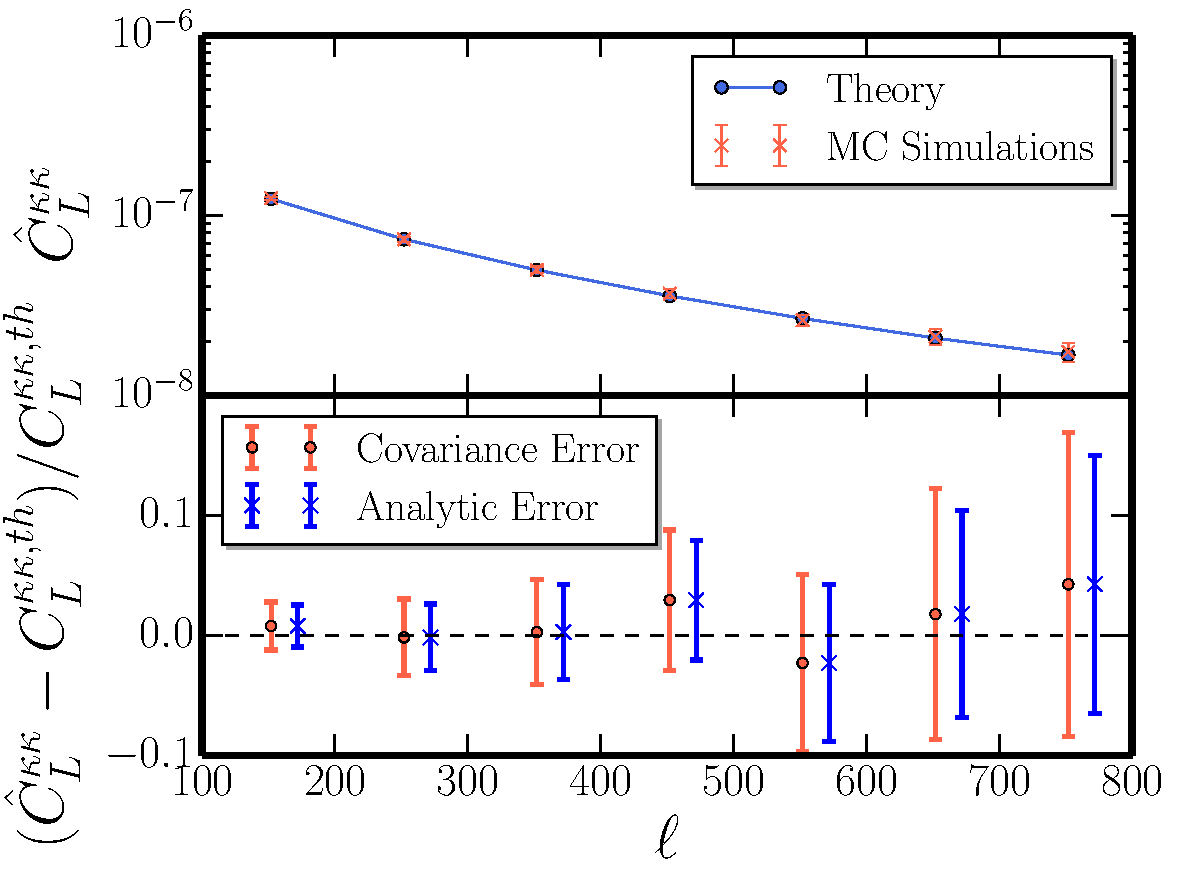
\includegraphics[scale=0.4]{Chapter3/Images/f8}
\caption{\emph{Left}. \emph{Upper panel}: cross-power spectrum of simulated galaxy and lensing maps constructed with $b=3$. The points connected by the solid blue line represent the binned input cross-spectrum, and the average reconstructed spectrum from 500 simulations is shown by the orange points. \emph{Lower panel}:  fractional difference between the input and extracted cross-spectra. Error bars obtained with the simulation covariance matrix (orange points) and with the analytical approximation (blue points) are shown for comparison. \emph{Middle}. As in left plot, but for the galaxy auto-power spectrum. \emph{Right}. As in left plot, but for the \gls{CMB} convergence autopower spectrum}
\label{fig:validation}
\end{figure*}

%%%%%%%%%%%%%
%%  RESULTS		  %%
%%%%%%%%%%%%%

\section{Power spectra}
\label{sec:power_spectraxc1}

\subsection{CMB Convergence-Galaxy Cross-correlation}
\label{subsec:kg_resultsxc1}

The recovered cross-spectrum is shown in Fig.~\eqref{fig:kg_all_mag}.  To compute it we have applied to both maps masks that select the five H-ATLAS patches of interest. The error bars are estimated by cross-correlating 500 \gls{MC} realizations of simulated \gls{CMB} convergence maps (consisting of both signal and noise) with the true H-ATLAS galaxy density map, as described in Sec \eqref{subsec:null_testsxc1}. This method (\gls{MC}1 in the language of Ch.~\eqref{sec:cov_est}) assumes that the two maps are uncorrelated; our error estimates are a good approximation because both maps are very noisy and $C_{\ell}^{\kappa\kappa,\rm tot}C_{\ell}^{gg,\rm tot}\gg (C_{\ell}^{\kappa g})^2$. We have also estimated the errors from cross-correlations of 500 \gls{MC} realizations of simulated H-ATLAS galaxy density maps with the real \textit{Planck} \gls{CMB} convergence map. The former approach yields slightly smaller error bars, yet slightly larger than those estimated analytically (see Fig. \eqref{fig:kg_errors}). These error estimates were checked by cross-correlating  the publicly available set of 100 simulated lensing maps, which accurately reflect the \emph{Planck} noise properties, with the real H-ATLAS map. The derived error bars are comparable with those found with our baseline approach, and there is no sign of systematic under- or overestimation.

\begin{figure}%9
\centering % \begin{center}/\end{center} takes some additional vertical space
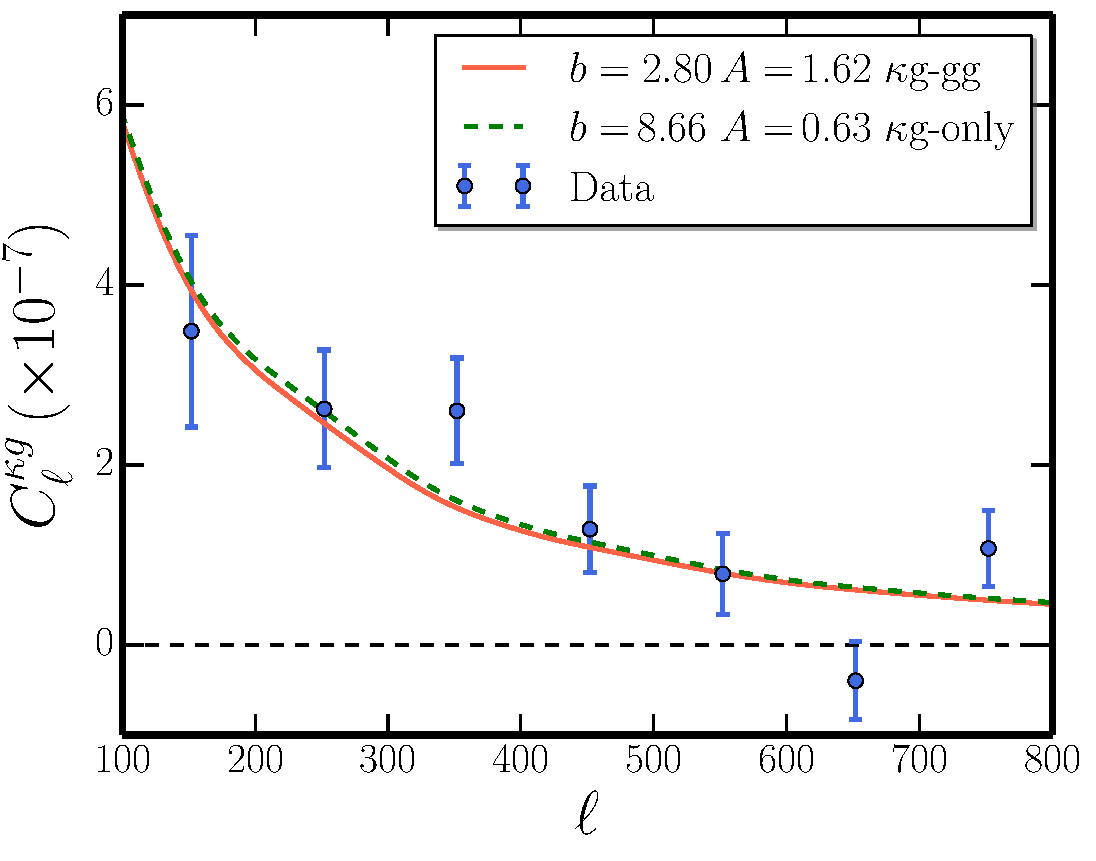
\includegraphics[width=0.6\textwidth]{Chapter3/Images/f9}
%\epsscale{0.5}
\caption{The \gls{CMB} convergence-galaxy density cross-spectrum as measured from Planck and \textit{Herschel} data. The data points are shown in blue, with error bars computed using the full covariance matrix obtained from Monte Carlo realizations of convergence maps. The theoretical spectra calculated with the bias values inferred from the likelihood analysis (as described in text) using the cross-correlation data only (solid red line) and the cross-correlation together with the galaxy autocorrelation data (dot-dashed green line) are also shown; we fix $\alpha=3$ in this analysis. The null (no correlation) hypothesis is rejected at the $20\,\sigma$ level.  \label{fig:kg_all_mag}}
\end{figure}


\begin{figure} %10
\centering % \begin{center}/\end{center} takes some additional vertical space
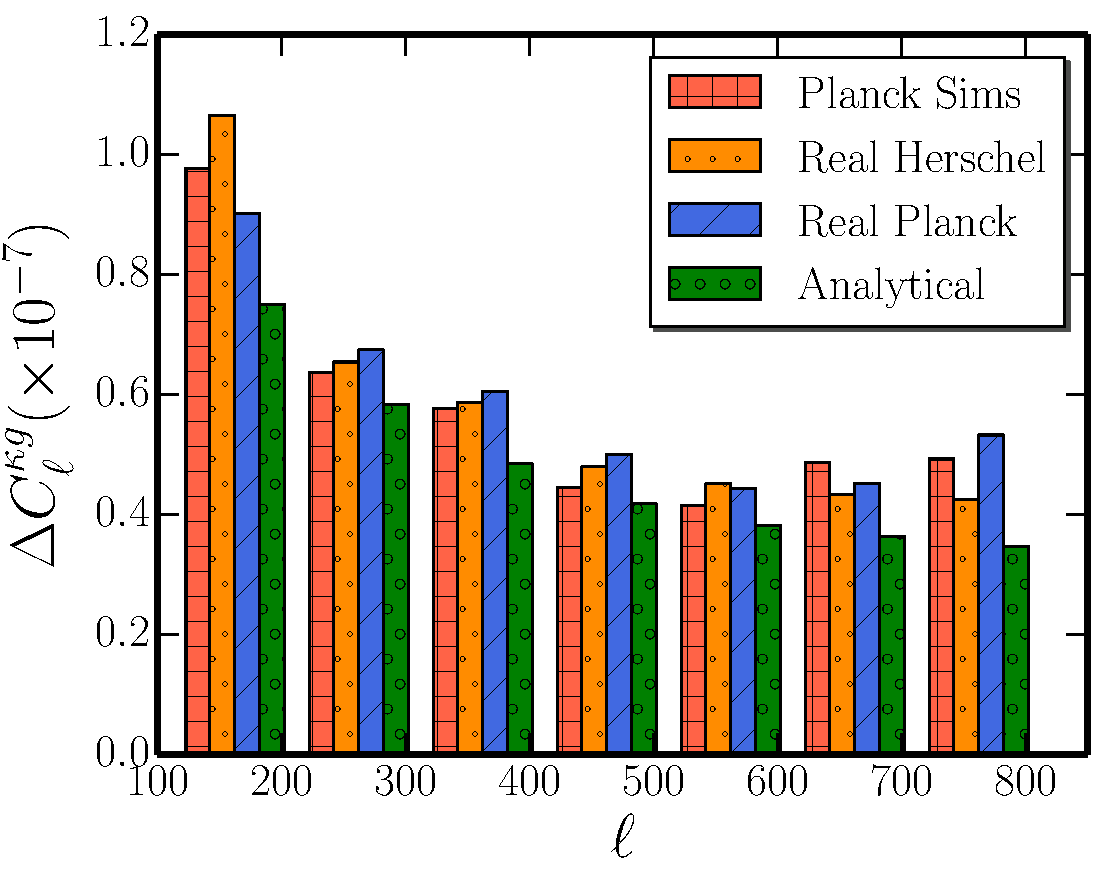
\includegraphics[width=0.6\textwidth]{Chapter3/Images/f10}
\caption{Error estimates for the cross-power spectrum band powers. The Monte Carlo estimates associated with estimated band powers are shown in orange ($500$ simulated lensing maps correlated with the real galaxy field).  Blue bars represent errors obtained by correlating $500$ simulated galaxy maps  with the real convergence field, and the green bars represent the analytical approximation to these errors. Error estimates obtained by correlating the real galaxy field with the 100 lensing simulated maps by the Planck collaboration are shown in red. \label{fig:kg_errors}}
\end{figure}


\begin{figure} %11
\centering % \begin{center}/\end{center} takes some additional vertical space
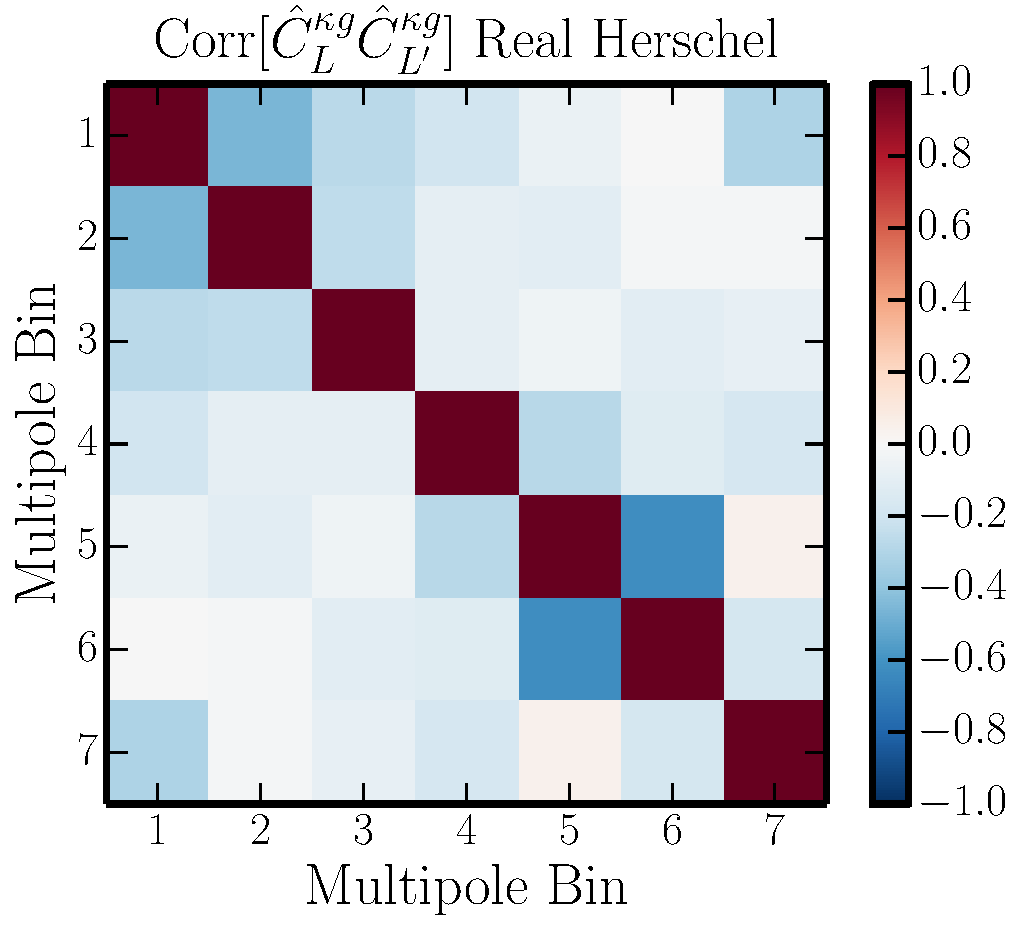
\includegraphics[width=0.6\textwidth]{Chapter3/Images/f11}
\caption{Correlation matrix Corr$[\hat{C}^{\kappa g}_{L} \hat{C}^{\kappa g}_{L'} ]$ built from the covariance matrix obtained by correlating $500$ simulated lensing maps with the real H-ATLAS galaxy map. \label{fig:corr_kg}}
\end{figure}

We have exploited the simulations to build the covariance matrix, used to evaluate the probability that the measured signal is consistent with no correlation (our null hypothesis). As can be seen in Fig.~\eqref{fig:corr_kg}, the covariance matrix is dominated by the diagonal components; however, off-diagonal components are non-negligible and have to be taken into account. The $\chi^2$ was calculated as
\begin{equation}
\chi_{\text{null}}^2 = \hat{\mathbf{C}}^{\kappa g}_{L} \,(\text{Cov}^{\kappa g}_{LL'})^{-1}\, \hat{\mathbf{C}}^{\kappa g}_{L'}.
\end{equation}
%
For the analysis performed with the whole H-ATLAS sample we obtained $\chi_{\rm null}^2 = 83.3$ for $\nu = 7$ degrees of freedom (dof), corresponding to a probability that the null hypothesis holds of $p=2.89 \times 10^{-15}$.  Because the $\chi^2$ distribution has mean $\nu$ and variance $2\nu$, the null hypothesis is rejected with a significance of about $(83.3-7)/(14^{1/2})\simeq 20\,\sigma$. This is the sum in quadrature of the significance of the correlation in each band power, taking into account the correlations between different bins. The results of the $\chi^2$ analysis for each patch are reported in Table \eqref{kg_sigma}.

\subsection{Galaxy Autocorrelation}\label{sec:autocorrxc1}
We also performed an analysis of the autocorrelation of \textit{Herschel} galaxies on the different patches. The shot noise subtracted autopower spectrum measured for the complete H-ATLAS data set is shown in Fig. \eqref{fig:gg_data_all}. The error bars on the data points are evaluated from the diagonal part of the covariance matrix built from galaxy simulations with bias $b=3$. The detected signal is highly significant ($40\,\sigma$).

\begin{figure} %12
\centering % \begin{center}/\end{center} takes some additional vertical space
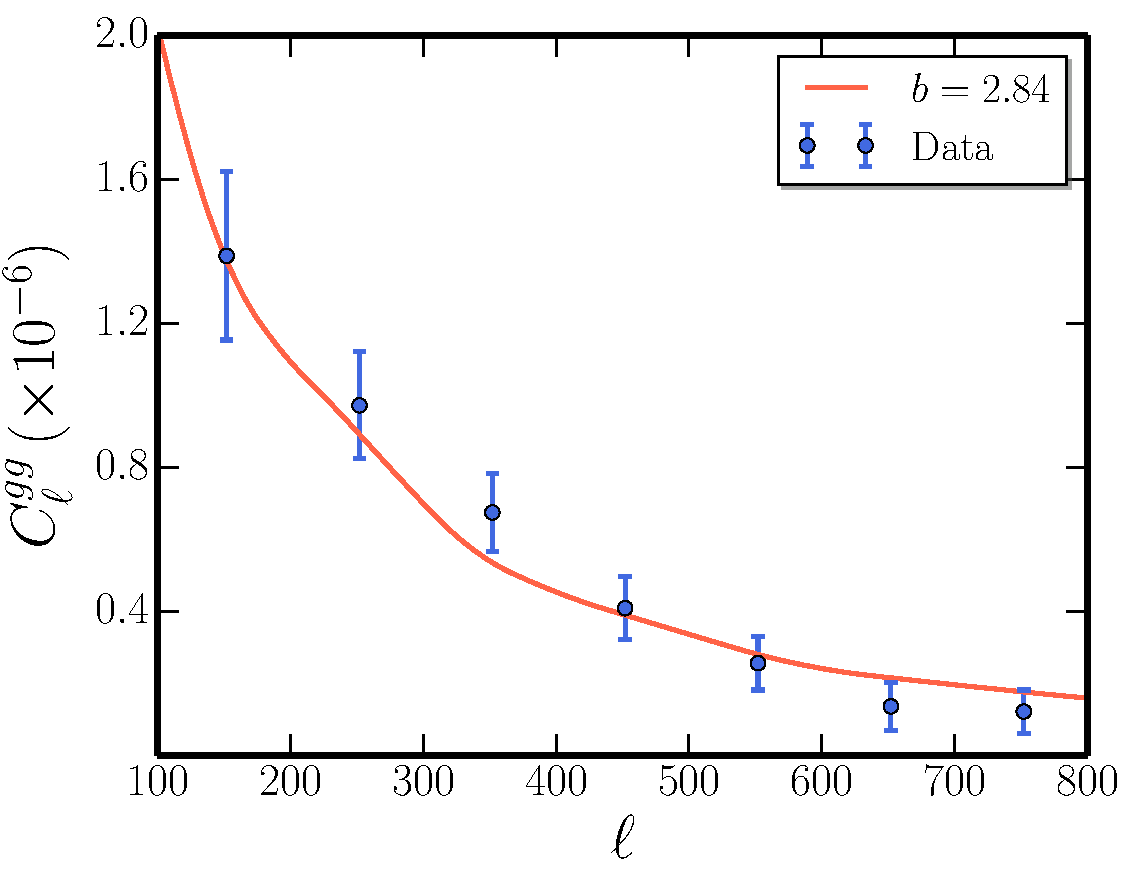
\includegraphics[width=0.7\textwidth]{Chapter3/Images/f12}
\caption{Galaxy density autopower spectrum for the whole sample of H-ATLAS galaxies. The data points are shown in blue, and the solid (red) line is the theoretical $C_{\ell}^{gg}$ evaluated for the best-fit value of the bias obtained using a likelihood analysis on the galaxy autospectrum data.\label{fig:gg_data_all}}
\end{figure}

\subsection{Null Tests}
\label{subsec:null_testsxc1}
In order to verify our pipeline and the reconstructed spectra against the possibility of residual systematic errors, we performed a series of null tests, which consist of cross-correlating the real map of one field with simulated maps of the other field. Because there is no common cosmological signal, the mean correlation must be zero.

We cross-correlated our $500$ simulated \gls{CMB} lensing maps (containing both signal and noise) with the real H-ATLAS galaxy density contrast map and our $500$ simulated galaxy maps constructed using $b=3$ with the true \emph{Planck}  \gls{CMB} convergence map. The error bars on the cross-power spectra were computed using the covariance matrices obtained from these simulations. As illustrated in Fig. \eqref{fig:null_tests} in both cases no significant signal was detected. In the first test we obtained $\chi^2 = 7.2$ corresponding to a probability of the null hypothesis (no correlation) $p=0.41$, and in the second one we have $\chi^2 = 5.9$ and $p=0.55$.

A further test consisted of cross-correlating the galaxy distribution in one patch of the sky with the lensing map in another. We moved in turn the three H-ATLAS GAMA fields and the SGP field to the position of the NGP patch and shifted  the NGP galaxies to the SGP area. Then we cross-correlated each shifted galaxy map with the convergence field in the same position. The errors on the cross-correlations were obtained as above. All of the cross-spectra are consistent with no signal.

\begin{figure} %13
\centering % \begin{center}/\end{center} takes some additional vertical space
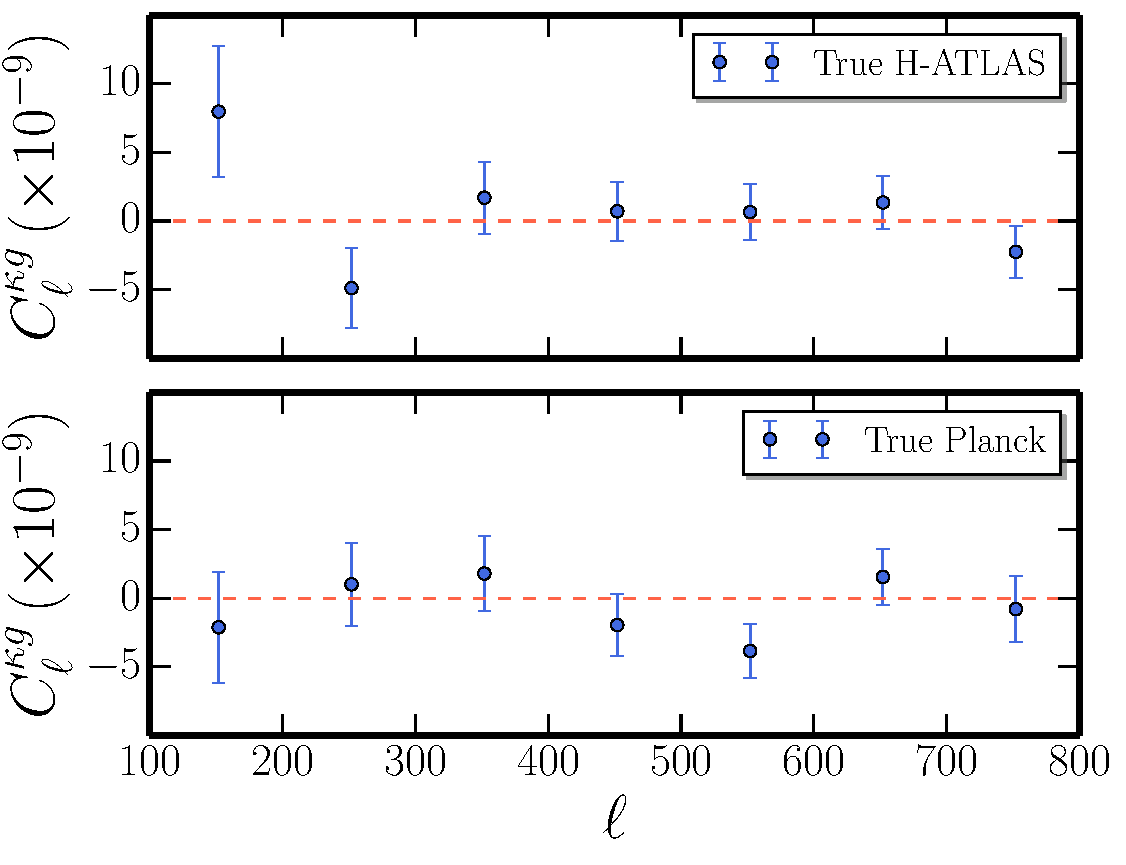
\includegraphics[width=0.7\textwidth]{Chapter3/Images/f13}
\caption{Results of null tests. \emph{Upper panel}: mean correlation between the true H-ATLAS map including all of the five patches and $500$ simulated \gls{CMB} lensing maps.
\emph{Lower panel}: mean cross-spectra between the true \emph{Planck} lensing map and $500$ simulated galaxy maps with $b=3$. No significant signal is detected in either case.
\label{fig:null_tests}}
\end{figure}

\begin{table}[t]
\centering
\begin{tabular}{cccc}
\toprule
\midrule
Patch & $\chi_{\text{null}}^2 / \nu$ & p-value & Significance\\
\midrule
ALL   &   $83.31/7 $&    $2.89 \times 10^{-15}  $ &    $20.3 \sigma$  \\
NGP  &   $34.03/7 $&    $1.70 \times 10^{-5}    $ &    $7.2 \sigma $ \\
SGP  &   $27.77/7 $&    $0.002                            $&    $5.6 \sigma $  \\
G09   &   $22.41/7 $&    $0.002                          $ &     $4.1 \sigma $ \\
G12   &   $22.26/7 $&    $0.002                           $ &   $4.1\sigma $  \\
G15   &   $29.23/7 $&    $1.0 \times 10^{-4}    $ &    $5.9 \sigma $ \\
\bottomrule
\end{tabular}
\caption{Significance of No Cross-correlation Hypothesis Rejection}
\label{kg_sigma}
\end{table}


%%%%%%%%%%%%%
%%  DISCUSSION	   %%
%%%%%%%%%%%%%
\section{Constraints on bias and amplitude of cross-correlation}
\label{sec:constraintsxc1}

We now discuss the cross-correlation signal of cosmological origin. We introduce a phenomenologically motivated parameter, $A$, that scales the expected amplitude of the cross-power spectrum, $C^{\kappa g}_{\ell}$, of the \emph{Planck} \gls{CMB} lensing with the H-ATLAS galaxy overdensity map as $A\, C^{\kappa g}_L(b)$. Obviously, its expected value is one. The introduction of such parameter enables consistency checks both at the data and theory level: deviations from unity might point toward an incorrect modeling of the signal (e.g. wrong redshift distribution estimate, scale-dependent bias and magnification bias), new physics (e.g. growth history different from assumed \gls{LCDM} and primordial NG) or systematics affecting the datasets (e.g. residual correlated contamination in the maps). Because the theoretical cross-spectrum is also basically proportional to the galaxy bias, there is a strong degeneracy between these two parameters. In order to break this degeneracy, we use also the galaxy autopower spectrum which depends only on $b$. 

Let us note that, depending on the subject of the study, previous works in literature adopted different strategies to interpret the cross-correlation signal. We can distinguish two main approaches: either the bias is fixed (or a bias template is assumed) from prior knowledge and the observed cross-spectrum $\hat{C}_{\ell}^{\kappa g}$ is fit for an amplitude parameter $A$ \citep{Sherwin2012,Ade2014c,Allison2015a,Giannantonio2016a}, or the cosmology is assumed to be known and the reconstructed cross-spectrum is fit for the bias value \citep{Feng2012,Bleem2012,Geach2013,DiPompeo2014,Omori2015}. Both estimated $A$ or $b$ can then be converted in derived parameters; in particular, it is possible to construct statistics sensitive to deviations from \gls{LCDM}, such as $E_g$ \citep{Pullen2016} and $D_g$ \citep{Giannantonio2016a}, by combining \gls{CMB} lensing-galaxy cross-spectra with galaxy auto-spectra. We stress that the analysis presented here is the first one that constrain the cross-correlation amplitude $A$ and linear galaxy bias $b$ by combining the two-point statistics $C_{\ell}^{\kappa g}$ and $C_{\ell}^{gg}$. This analysis scheme has been subsequently exploited by \cite{Kuntz2015} to reanalyze the cross-correlation signal between the CHFTLens galaxies with the \emph{Planck} \gls{CMB} lensing firstly studied by \cite{Omori2015}.
 
The best-fit values of the amplitude and of the galaxy bias were obtained by means of Bayesian analysis. In the following, we first describe the likelihood functions and present constraints on the redshift-independent galaxy bias and on the cross-correlation amplitude using galaxy autocorrelation data alone, cross-correlation data alone, and combining both data sets. In this analysis, the cosmological parameters and the counts slope $\alpha$ are kept fixed to the fiducial values. In order to efficiently sample the parameter space, we use the Markov chain Monte Carlo (MCMC) method assuming uninformative flat priors. For this purpose we employ \texttt{emcee} \citep{Foreman-Mackey2013}, a public implementation of the affine invariant MCMC ensemble sampler \citep{Goodman2010}.  In this chapter, each quoted parameter estimate is the median of the appropriate posterior distribution after marginalizing over the remaining parameters with uncertainties given by the $16^{\rm th}$ and $84^{\rm th}$ percentiles (indicating the bounds of a $68\%$ credible interval). For a Gaussian distribution, as is the case when combining both data sets, these percentiles correspond approximately to $-1\sigma$ and $+1\sigma$ values, and the median of the posterior is equal to the mean and maximum likelihood value.
%
\begin{table}[t]
\centering
\begin{tabular}{ccccccccccc}
\toprule
\midrule
 \multicolumn{1}{c}{}& \multicolumn{1}{c}{$gg$} &  \multicolumn{1}{c}{}& \multicolumn{2}{c}{$\kappa g$} &  \multicolumn{1}{c}{}&   \multicolumn{2}{c}{$\kappa g+gg$} & \multicolumn{1}{c}{} &\multicolumn{1}{c}{}  &   \\
\cline{2-2} \cline{4-5} \cline{7-8} \\
{Patch} & {$b$} & {} & {$b$} & {$A$} & {}  & {$b$} & {$A$} &  {} &  {$\chi^2_{\rm th}/\nu$} &  {p-value}\\
\midrule
ALL & $2.84 ^{+0.12}_{-0.11}$ &   & $8.66^{+4.23}_{-4.37}$ & $0.63^{+0.52}_{-0.20}$ &  & $2.80 ^{+0.12}_{-0.11}$ & $1.62 ^{+0.16}_{-0.16}$ &   & $12.6/5$ & $0.03$ \\
NGP & $2.72 ^{+0.22}_{-0.21}$ &   & $7.92^{+5.38}_{-6.38}$ & $0.53^{+1.35}_{-0.26}$ & & $2.75 ^{+0.22}_{-0.21}$ & $1.27 ^{+0.28}_{-0.29}$ &   & $23.1/5$ & $3 \times 10^{-4}$ \\
SGP & $2.67 ^{+0.19}_{-0.19}$ &   & $0.78^{+1.86}_{-0.61}$ & $3.48^{+2.63}_{-1.95}$ &  & $2.69 ^{+0.18}_{-0.18}$ & $1.56 ^{+0.23}_{-0.23}$ &   & $5.7/5$ & $0.34$ \\
G09 & $3.79 ^{+0.35}_{-0.37}$ &   & $8.99^{+4.02}_{-5.06}$ & $1.11^{+0.96}_{-0.36}$ &  & $3.72 ^{+0.35}_{-0.32}$ & $2.11 ^{+0.41}_{-0.41}$ &   & $6.9/5$ & $0.22$ \\
G12 & $3.43 ^{+0.35}_{-0.33}$ &   & $3.34^{+6.84}_{-2.55}$ & $2.04^{+3.41}_{-1.23}$ &  & $3.36 ^{+0.35}_{-0.33}$ & $2.05 ^{+0.47}_{-0.46}$ &   & $ 13.7/5$ & $0.02$ \\
G15 & $3.14 ^{+0.33}_{-0.35}$ &  & $8.57^{+4.85}_{-6.54}$ & $0.97^{+1.72}_{-0.38}$ &  & $3.13 ^{+0.34}_{-0.34}$ & $2.06^{+0.45}_{-0.47}$ &  & $18.4/5$ & $2\times 10^{-3}$ \\
\bottomrule
\end{tabular}
\caption{H-ATLAS galaxy linear bias and cross-correlation amplitude as determined using both separately and jointly the reconstructed galaxy auto- and cross-spectra in the different patches}
\label{b_a_results}
\end{table}
%{} & {$gg$} &  {} & \multicolumn{2}{c}{$\kappa g$} & {} &   \multicolumn{2}{c}{$\kappa g+gg$} &  {} &  {} &  {}  \\
%\cline{2-2} \cline{4-5} \cline{7-8} \\
%{Patch} & {$b$} & {} & {$b$} & {$A$} & {}  & {$b$} & {$A$} &  {} &  {$\chi^2_{\rm th}/\nu$} &  {p-value}}

We assumed Gaussian likelihood functions for the cross- and autopower spectra. For the galaxy autopower spectrum it takes the form

\begin{equation}
\label{eqn:like_gg}
\begin{split}
\mathcal{L}(\hat{C}^{gg}_{L}|b) &= \frac{1}{\sqrt{(2\pi)^{N_{L}}\det(\text{Cov}^{gg}_{LL'})}} \\
&\times \exp \Biggl\{ -\frac{1}{2} [\hat{C}^{gg}_{L} - C^{gg}_{L}(b)] \,(\text{Cov}^{gg}_{LL'})^{-1} \, [\hat{C}^{gg}_{L'} - C^{gg}_{L'}(b)]  \Biggr\},
\end{split}
\end{equation}
where $N_{L} = 7$ is the number of multipole bins and $\rm Cov^{gg}_{LL'}$ is the covariance matrix computed as described in Sec~\eqref{sec:covxc1}.

By sampling this likelihood for the measured H-ATLAS galaxy power spectrum $\hat{C}^{gg}_{L}$ we obtained constraints on the galaxy bias. Estimated values of the bias for all patches as well as for each of them  are presented in Table~\eqref{b_a_results}. The results for the different patches are consistent with each other within $\lesssim 2\sigma$ and we note the GAMA patches to be appear a bit more biased with respect to NGP and SGP. The global value, $b=2.84\pm 0.12$, is consistent with earlier estimates. For example, \cite{Xia2012} found an effective value of the bias factor $b_{\rm eff}\simeq 3$ (no error given) "for the bulk of galaxies at $z\simeq 2$''. The \cite{Ade2014h} found, from their analysis of the CIB, a slightly lower value ($b_{\rm eff}\simeq 2.6$), as expected because a large contribution to the CIB comes from fainter, presumably less biased, sources.

We used the measured cross-spectra to constrain the $b$ and $A$ parameters in the same fashion. As noted above, the cross-spectra basically measure the product $A\times b$. The likelihood function is given by
\begin{equation}
\label{eqn:like_kg}
\begin{split}
\mathcal{L}(\hat{C}^{\kappa g}_{L}|b,A) &= \frac{1}{\sqrt{(2\pi)^{N_{L}}\det(\text{Cov}^{\kappa g}_{LL'})}}\\
&\times \exp \Biggl\{ -\frac{1}{2} [\hat{C}^{\kappa g}_{L} - A\,C^{\kappa g}_{L}(b)] \,(\text{Cov}_{LL'}^{\kappa g})^{-1} \, [\hat{C}^{\kappa g}_{L'} - A\,C^{\kappa g}_{L'}(b)]  \Biggr\},
\end{split}
\end{equation}
where $\rm Cov^{\kappa g}_{LL'}$ is the covariance matrix (Eq.~(\eqref{eqn:analytic_covariance})). The results are shown in Table \eqref{b_a_results}.

Finally, we studied the constraints on $b$ and $A$ by combining the cross- and galaxy autospectra. For the joint analysis we used the Gaussian likelihood function that takes into account correlations between the cross- and the autopower spectra in the covariance matrix. We organized the extracted cross- and autoband powers into a single data vector as
\begin{equation}
\mathbf{\hat{C}}_{L} = (\mathbf{\hat{C}}^{\kappa g}_{L}, \mathbf{\hat{C}}^{gg}_{L}),
\end{equation}
which has 14 elements. The total covariance matrix is then written as the composition of four $7\times7$ submatrices
\begin{equation}
\text{Cov}_{LL'} =
\begin{bmatrix}
\text{Cov}^{\kappa g}_{LL'} & (\text{Cov}^{\kappa g-gg}_{LL'})^\intercal \\
 \text{Cov}^{\kappa g-gg}_{LL'} & \text{Cov}^{gg}_{LL'}  \\
\end{bmatrix}
\end{equation}
where the mixed covariance that takes into account the correlation between the two observables is
\begin{align}
 \text{Cov}^{\kappa g-gg}_{LL'} &= M_{LL_1}^{-1}P_{L_1\ell}\widetilde{\text{Cov}}^{\kappa g-gg}_{\ell\ell'}Q_{\ell'L_2}(M_{L'L_2}^{-1})^\intercal \\
{\widetilde{\text{Cov}}^{\kappa g-gg}_{\ell\ell'}} &= \frac{2}{2\ell'+1} 
M_{\ell\ell'}\bigl[(C^{gg}_{\ell}(b)+N^{gg}_{\ell})(C^{gg}_{\ell'}(b)+N^{gg}_{\ell'})C^{\kappa g}_{\ell}(b)C^{\kappa g}_{\ell'}(b) \bigr]^{1/2}.
\end{align}
In the above expressions, $\text{Cov}^{\kappa g}_{LL'}$ and $\text{Cov}^{gg}_{LL'}$ are the covariance matrices evaluated using Eq.~(\eqref{eqn:analytic_covariance}).

The full 2-dimensional posterior distributions of the $b$ and $A$ parameters, as well as the marginalized ones obtained from this analysis, are shown in Fig.~\eqref{fig:kg_gg_pdf}. Numerical values of the parameters are presented in Table \eqref{b_a_results}, where the best-fit values and the errors are evaluated as the $50^{\rm th}$, $16^{\rm th}$, and $84^{\rm th}$ percentiles, respectively, of the posterior distributions. The $\chi^2$ values are evaluated as $\chi^2_{\rm th} = [\hat{\mathbf{C}}^{\kappa g}_L - A_{\rm bf}\mathbf{C}^{\kappa g}_L(b_{\rm bf})] (\text{Cov}^{\kappa g}_{LL'})^{-1}$ $[\hat{\mathbf{C}}^{\kappa g}_{L'} - A_{\rm bf}\mathbf{C}^{\kappa g}_{L'}(b_{\rm bf})] $, where $b_{\rm bf}$ and $A_{\rm bf}$ are the best-fit values. Note that the posterior distributions of $b$ and $A$ obtained using only cross-correlation data are far from being Gaussian. As a sanity check, we derived a theoretical upper limit on $A$ considering that cross-spectrum cannot be larger than the geometric mean of the two autospectra: $A \le (C^{\kappa g, \rm th}_L \rm (Cov^{\kappa g}_{LL'})^{-1} \sqrt{\hat{C}^{\kappa\kappa}_{L'}\hat{C}^{gg}_{L'}})/(C^{\kappa g, \rm th}_L \rm (Cov^{\kappa g}_{LL'})^{-1} C^{\kappa g, \rm th}_{L'}) \sim 2.5$. 

\begin{figure} %14
\centering % \begin{center}/\end{center} takes some additional vertical space
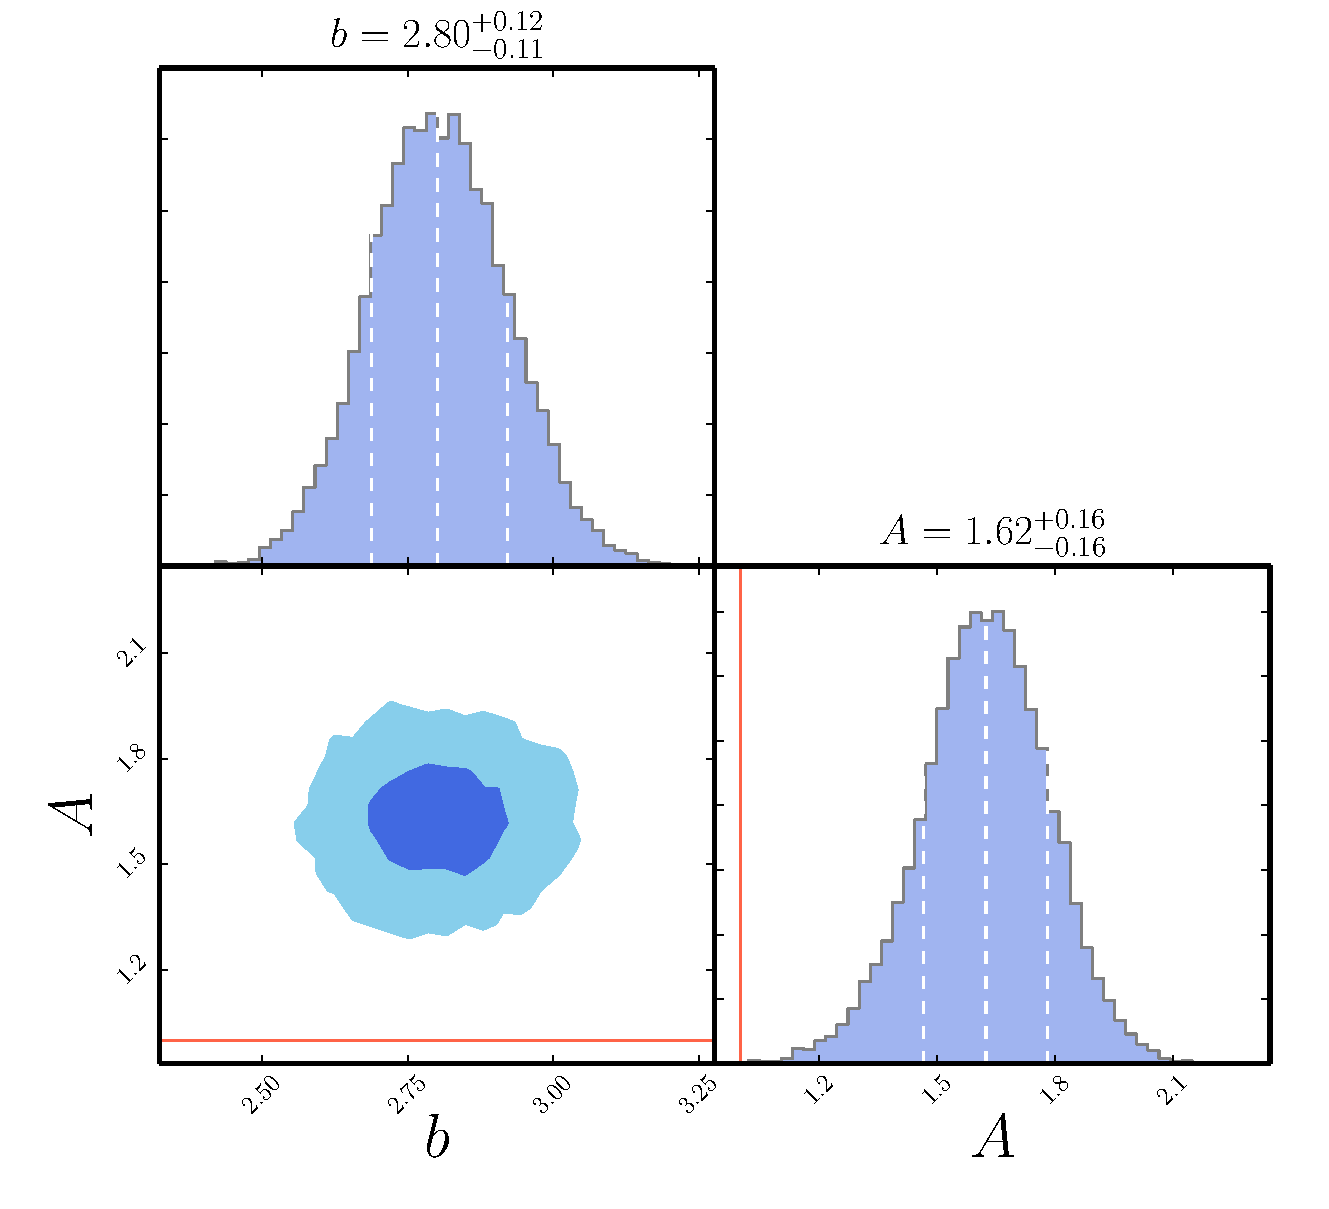
\includegraphics[width=0.8\textwidth]{Chapter3/Images/f14}
\caption{Posterior distribution in the $b-A$ plane with the 68\% and 95\% confidence contours (darker and lighter colors, respectively), together with the marginalized distributions of each parameter with $1\sigma$ errors shown by the dashed white lines, obtained by combining the convergence-galaxy cross-correlation and the galaxy autocorrelation data for each patch. The solid red line represents the standard case in which $A=1$, and $\alpha$ is set to 3 for the analysis. \label{fig:kg_gg_pdf}}
\end{figure}

The $\chi^2$ value of the best-fit theoretical spectrum is $\chi^2_{\rm th} = 12.6$ for $\nu=5$ dof  ($\chi^2_{\rm th}/\nu = 2.5$). The significance of the detection of the theoretically expected cross-correlation signal was  evaluated as the ratio between the estimated amplitude $A$ and its error $\sigma_A$: $A/\sigma_A \simeq 10$, corresponding to a $10\sigma$ significance.

The constraint on the bias factor from the joint fit of the galaxy autocorrelation and of the cross-correlation power spectra, $b=2.80^{+0.12}_{-0.11}$, is consistent with earlier estimates \citep{Xia2012}. On the other hand, the cross-correlation amplitude is $A=1.62\pm 0.16$ times larger than expected for the standard $\Lambda$CDM model for the evolution of large-scale structure. This is at odds with the results of the cross-correlation analyses presented in the \cite{Ade2014c} paper, which are consistent with $A=1$ except, perhaps, in the case of the MaxBCG cluster catalog. Possible causes of the large value of $A$ are discussed in the following section.

In order to provide further proof of the reliability of the MCMC analysis, as well as to give a comparison of the constraining power of the different two-point statistics exploited here, we conclude this subsection with Fig.~\eqref{fig:kg_gg_correct}: there, we show the results of the MCMC analysis on mock data using $C_{\ell}^{gg}$, $C_{\ell}^{\kappa g}$, and $C_{\ell}^{gg} + C_{\ell}^{\kappa g}$. To produce this plot we first output two correlated \textit{signal plus noise} $\kappa$ and $g$ maps with the fiducial model by setting $b=3$  and $A=1$. We then extract both the cross- and auto-power spectra and fit separately $\hat{C}_{\ell}^{gg, \rm{fake}}$ and $\hat{C}_{\ell}^{\kappa g, \rm{fake}}$ (assuming $A=1$) for the bias value, while the combination of $\hat{C}_{\ell}^{\kappa g, \rm{fake}} + \hat{C}_{\ell}^{gg, \rm{fake}}$ is fit for the bias and amplitude parameters. As we can see, in all cases the input model is recovered, i.e. $b=3$ and $A =1$ within 1$\sigma$, and there are no signs of spurious biases. In particular, the galaxy auto-power spectrum seems to constrain tighter the value of the linear galaxy bias, though it is expected to be much more sensitive to residual systematics.

\begin{figure} %14
\centering % \begin{center}/\end{center} takes some additional vertical space
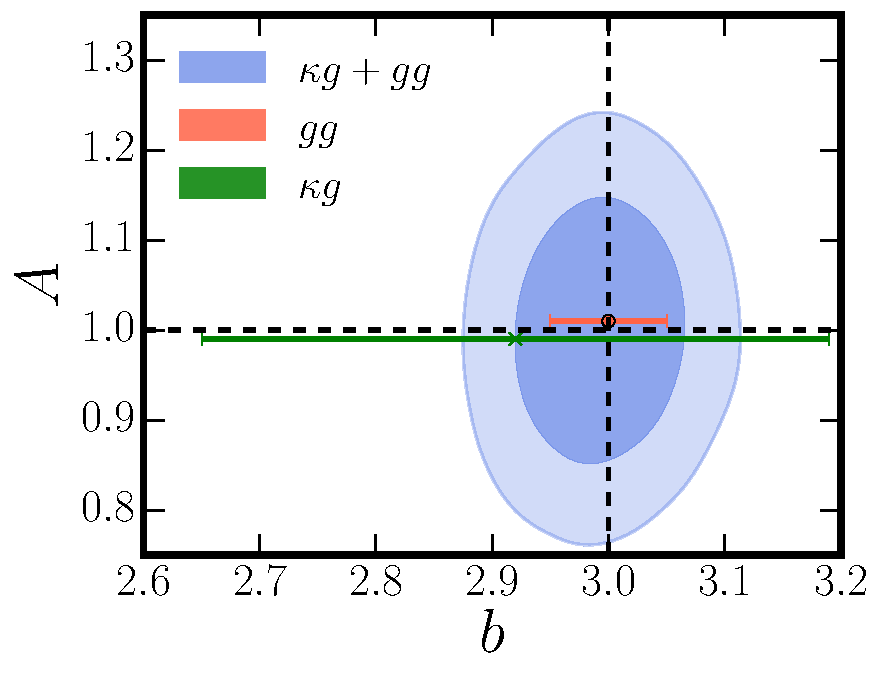
\includegraphics[width=0.7\textwidth]{Chapter3/Images/b_A_correct}
\caption{Validation of the MCMC pipeline and constraining power comparison. We show posterior distribution in the $b-A$ plane with the 68\% and 95\% confidence contours (darker and lighter colors, respectively), obtained by combining the \gls{CMB} convergence-galaxy cross-correlation and the galaxy autocorrelation mock data with $b=3$ and $A=1$. The $1\sigma$ red and green error bars represent the bias constraints found using only the $C_{\ell}^{gg}$ and $C_{\ell}^{\kappa g}$ (fixing $A=1$), respectively. \label{fig:kg_gg_correct}}
\end{figure}

\section{Discussion} \label{sec:discussionxc1}

The correlation between the \gls{CMB} lensing potential and the distribution of high-$z$, submillimeter selected galaxies was found to be stronger than expected for the standard cosmological model. We now address on one side the possibility that the tension between the estimated and the expected value of the amplitude $A$ is overrated because of an underestimate of  the errors and, on the other side, astrophysical effects that may enhance the measured signal.

\subsection{Noise Levels}

Due to the inhomogeneity of the noise level in the \emph{Planck} survey, the H-ATLAS patches used for the cross-correlation may have slightly higher than average effective noise. To check this possibility, we reconstructed the \gls{CMB} convergence autopower spectrum for each of the H-ATLAS patches. Error bars were derived from 100 simulated \emph{Planck} lensing maps.  The results of the analysis performed combining the five patches show some excess power for $\ell \sim 400$--500  (Fig.~\eqref{fig:kk_data_patches}). Considering the patches separately we find that the main features of the \gls{CMB} lensing power spectrum are recovered in the two largest patches, whereas the power spectrum in the three GAMA fields seems to be dominated by noise. Thus, there is an indication of a slight underestimate of the noise bias in the latter fields, but the effect on the combined patches is marginal.

\begin{figure} %15
\centering % \begin{center}/\end{center} takes some additional vertical space
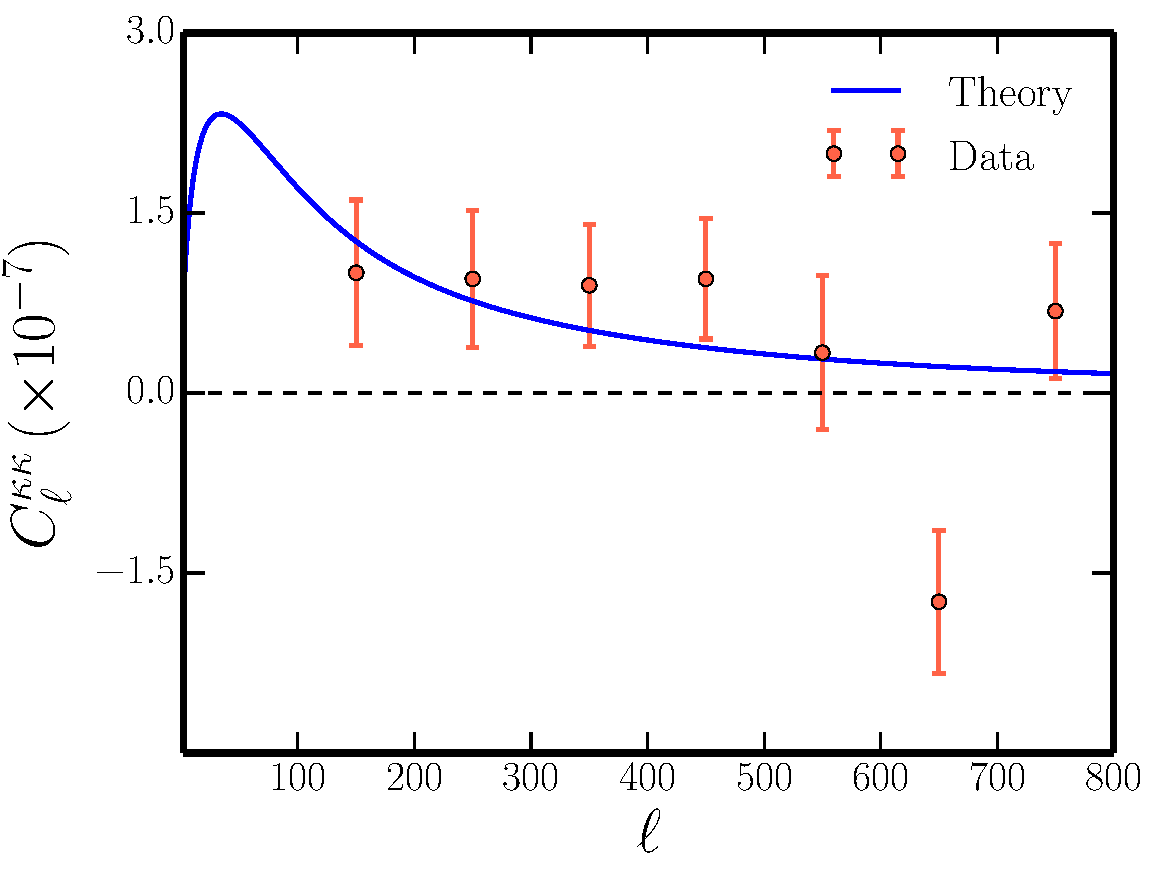
\includegraphics[width=0.7\textwidth]{Chapter3/Images/f15}
\caption{\gls{CMB} convergence autopower spectrum recovered using the H-ATLAS mask. Theory line as in Fig.~\eqref{fig:kk_data_planck}. \label{fig:kk_data_patches}}
\end{figure}

To understand which is the main statistical error source on the cross-power spectrum, we have analyzed the contributions to the error budget. The autospectra contain a signal and a noise term as $\hat{C}^{XX}_{L} = C^{XX}_{L}+N^{XX}_L$, so that the errors on the cross-spectra can be written as
%
\begin{equation}\label{eq:err_budget}
\begin{split}
f_{\rm{sky}}(2L+1)\Delta\ell \bigl(\Delta\hat{C}^{\kappa g}_L \bigr)^2 &= \bigl[C_{L}^{\kappa\kappa} C_{L}^{gg} + (C_{L}^{\kappa g})^2 \bigr]\\
&+ N^{\kappa\kappa}_LN^{gg}_L + C_{L}^{\kappa\kappa}N^{gg}_L + C_{L}^{gg}N^{\kappa\kappa}_L.
\end{split}
\end{equation}
%
The first term represents the cosmic variance, the second one the pure noise, and the remaining are mixed signal-noise terms. As can be seen from Fig.~\eqref{fig:noise_budget}, the main contribution to the $C^{\kappa g}_L$ variance is given by the noise-only term. Moreover, the relative amplitude of the mixed terms is telling us that most of the error comes from the lensing noise. In order to reduce the errors of the reconstructed cross-spectrum, it is important to reach high sensitivity in reconstructing the \gls{CMB} lensing potential. This, of course, does not include the possible systematic errors discussed below.

\begin{figure} %16
\centering % \begin{center}/\end{center} takes some additional vertical space
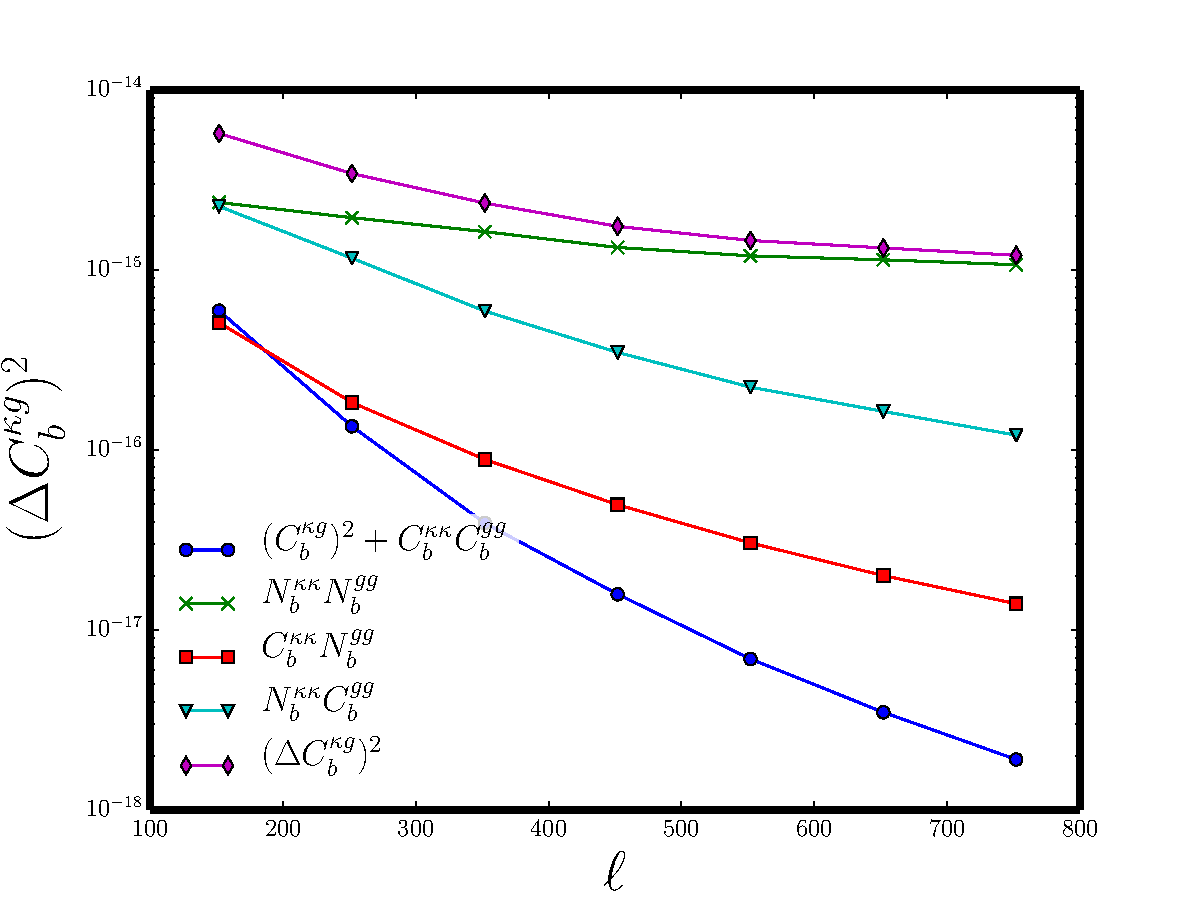
\includegraphics[width=0.7\textwidth]{Chapter3/Images/f16}
\caption{Contributions to the cross-spectrum variance $(\Delta {C^{\kappa g}_{\ell}})^2$ [see Eq.~(\eqref{eq:err_budget})]. Blue line: signal only term.  Green line: noise only term. Red and cyan lines: mixed signal and noise terms. \label{fig:noise_budget}}
\end{figure}


\subsection{Astrophysical systematics}

First we have checked the effect on the auto- and cross-spectra of errors of photometric redshift estimates. To this end we have redone the full analysis using the initial redshift distribution, $dN/dz$, i.e. the one represented by the dashed red line in Fig.~\eqref{fig:dndzxc1}. As shown in Fig.~\eqref{fig:kg_gg_un_convolved_pdf}, we get a slightly higher value of the cross-spectrum amplitude ($A=1.70^{+0.16}_{-0.17}$) and a somewhat lower value of the galaxy bias ($b=2.59^{+0.11}_{-0.11}$). The reason for that is easily understood. As shown by Fig.~\eqref{fig:dndzxc1}, the convolution of the initial $dN/dz$ with the smoothing kernel (representative of the uncertainties on estimated redshifts) results in a broadening of the distribution. This translates into a decrease of the expected amplitude for both the cross- and the autopower spectra. Hence, in order to fit the same data, we need a higher value of the galaxy bias and, consequently,  a lower value of the cross-spectrum amplitude $A$. Because the derived value of $b$ is quite sensitive to the adopted redshift distribution, the agreement with other, independent determinations implies that our $dN/dz$ cannot be badly off. Therefore, it looks unlikely that the higher than expected value of $A$ can be ascribed to a wrong estimate of $dN/dz$.

\begin{figure*} %17
\centering % \begin{center}/\end{center} takes some additional vertical space
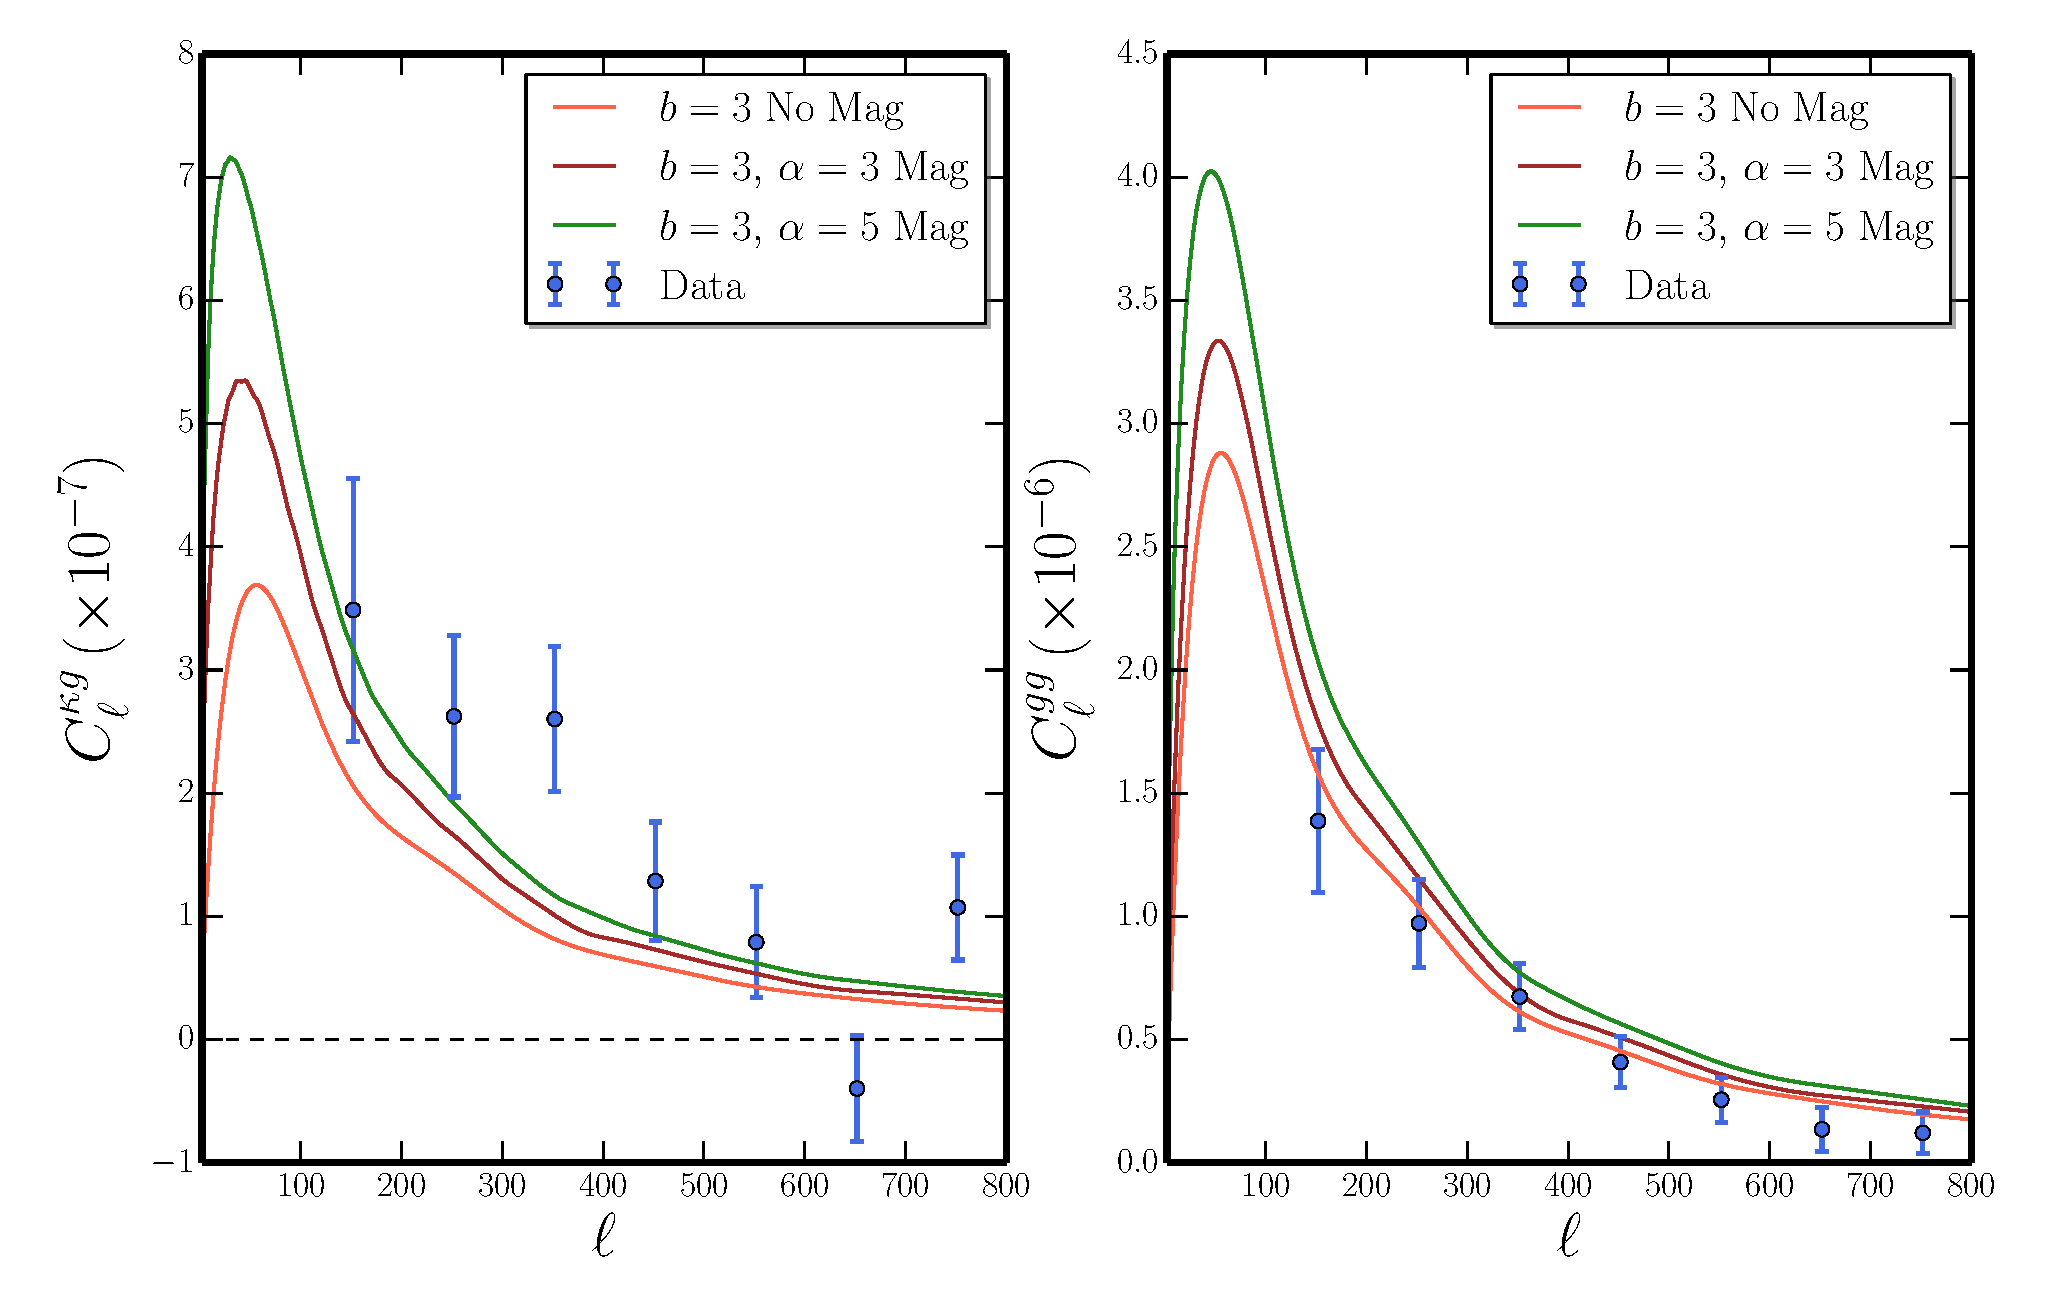
\includegraphics[width=0.7\textwidth]{Chapter3/Images/f17}
\caption{Effect of lensing magnification bias on the cross-power spectrum (left panel) and on the galaxy autopower spectrum (right panel).  In both panels, theory lines are plotted for bias values $b=3$, while the slope of the galaxy number counts as function of flux is set to $\alpha=1$ (no magnification) and $\alpha=3,5$ as described in the legend. \label{fig:kg_gg_mag_bias}}
\end{figure*}

Our choice of a constant $b$ over the redshift range spanned by the H-ATLAS catalog is obviously an approximation, and the effective values of $b$ may be different for the cross- and the galaxy autopower spectra. To check the effect of this approximation on the estimates of $C_{\ell}^{\kappa g}$ and $C_{\ell}^{gg}$ we have computed the effective values of the bias for the two cases
%
\begin{equation}
\label{eqn:b_eff}
\begin{split}
b_{\rm eff}^{\kappa g} &= \frac{\int \,\frac{\diff z}{c}b(z)\frac{H(z)}{\chi^2(z)}W^{\kappa}(z)\frac{dN}{dz}P_{\delta\delta}(k,z)}{\int\frac{\diff z}{c}\frac{H(z)}{\chi^2(z)} W^{\kappa}(z)\frac{dN}{dz}P_{\delta\delta}(k,z)},\\
(b_{\rm eff}^{gg})^2 &= \frac{\int \,\frac{\diff z}{c}b^2(z)\frac{H(z)}{\chi^2(z)}(\frac{dN}{dz})^2P_{\delta\delta}(k,z)}{\int\frac{\diff z}{c}\frac{H(z)}{\chi^2(z)}(\frac{dN}{dz})^2 P_{\delta\delta}(k,z)},
\end{split}
\end{equation}
%
using the bias evolution model $b(z)$ from \cite{Sheth1999} for halo masses in the range $10^{12}\hbox{--} 10^{13}\,\hbox{M}_{\odot}$. We find that $b_{\rm eff}^{\kappa g}$ is only slightly larger (by $\simeq 6\%$) than $b_{\rm eff}^{gg}$. Hence, considering a redshift-dependent bias factor would only marginally affect the expected cross-spectrum.


Weak lensing by foreground structures modifies the \textit{observed} density of background sources compared to the real one \citep{Ho2008,Xia2009} and is especially important for high-redshift objects. The effect on the galaxy overdensity kernel is described by the second term on the right-hand side of Eq.~(\eqref{eqn:wgxc1}). The effect of the magnification bias on both $C_{\ell}^{\kappa g}$ and $C_{\ell}^{gg}$ is illustrated in  Fig.~\eqref{fig:kg_gg_mag_bias} where we show the expected power spectra for $A=1$, $b=3$, and three values of $\alpha$: 1 (no magnification bias), 3, and 5. The impact of the magnification bias is clearly stronger for $C_{\ell}^{\kappa g}$.

Fitting the joint data for $\alpha=1$ we find  $b=2.95^{+0.12}_{-0.11}$ and  $A=1.93^{+0.18}_{-0.19 }$ while for $\alpha=5$, $b=2.55^{+0.13}_{-0.12}$ and  $A=1.46 \pm 0.14$. The contour plots in the $A-b$ plane are shown in Fig.~\eqref{fig:kg_gg_alphas_pdf}. Higher values of $\alpha$ imply lower values of $A$, but even for $\alpha = 5$ the data require $A>1$.

\begin{figure} %18
\centering % \begin{center}/\end{center} takes some additional vertical space
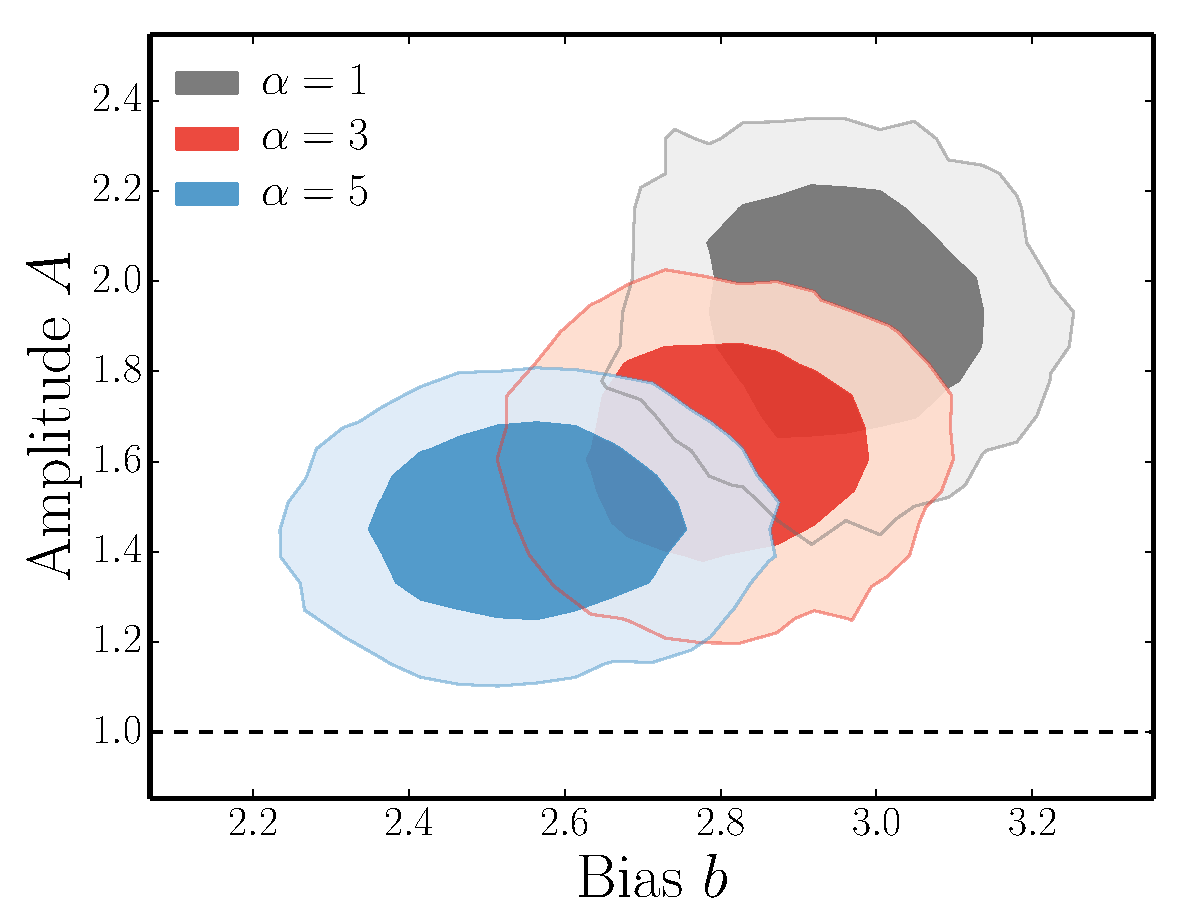
\includegraphics[width=0.7\textwidth]{Chapter3/Images/f18}
\caption{Effect of fixed slope of number counts $\alpha$ on the inferred values of cross-correlation amplitude $A$ and bias $b$. We show $1-$ and $2\sigma$ contours (darker and lighter shaded regions, respectively). As the $\alpha$ parameter increases, both $A$ and $b$ shift toward smaller values. \label{fig:kg_gg_alphas_pdf}}
\end{figure}

Another systematic effect that can bias our measurement of the \gls{CMB} convergence-galaxy cross-correlation is the leakage of \gls{CIB} emission into the lensing map through the temperature maps used for the lensing estimation, as it correlates strongly with the \gls{CMB} lensing signal \cite{Ade2014a}. The 857\,GHz \emph{Planck} map used by \cite{Ade2014c} as a Galactic dust template also removes the portion of the CIB fluctuations that have a spectral index similar to that of Galactic dust. However, as noted in that paper, this approach is liable to problems due, for example, to variation of Galactic dust spectral indices across the sky, as well as to the mismatch between the beams at 100/143/217 and 857 GHz.

The H-ATLAS galaxies are well below the \emph{Planck} detection limits (their flux densities at 148\,GHz are expected to be in the range 0.1--1\,mJy, hence are much fainter than sources masked by \cite{Ade2014c}). Thus they are part of the CIB measured by \emph{Planck}. If they are only partially removed by the use of the 857\,GHz map, they are potentially an important contaminant of the cross-correlation, resulting in an enhancement of the observed signal. The shot-noise correction applied by the \emph{Planck} analysis removes only partly the contamination by infrared sources because their main contribution to the fluctuation field is due to clustering.

Foreground induced biases to CMB lensing reconstruction have been extensively studied by \cite{VanEngelen2014} and \cite{Osborne2014}. These authors concluded that the impact of these sources of systematic errors should be small due to \emph{Planck}'s resolution and noise levels. However, a calculation of the bias on the cross-spectrum discussed in this chapter is beyond the scope of the present chapter.  Having at hand \gls{CMB} lensing maps at different frequencies would allow to investigate the CIB leakage issue in more detail.

Clusters of galaxies, which trace the large-scale potential responsible for the \gls{CMB} lensing, are visible at millimeter and submillimeter wavelengths via the scattering of \gls{CMB} photons by hot electrons {(Sunyaev-Zel'dovich effect)} and might therefore contaminate the cross-correlation signal to some extent. However, the redshift range populated by galaxy clusters only marginally overlaps with the redshift distribution of our sources, so that this contamination is negligible.

\begin{figure} %19
\centering % \begin{center}/\end{center} takes some additional vertical space
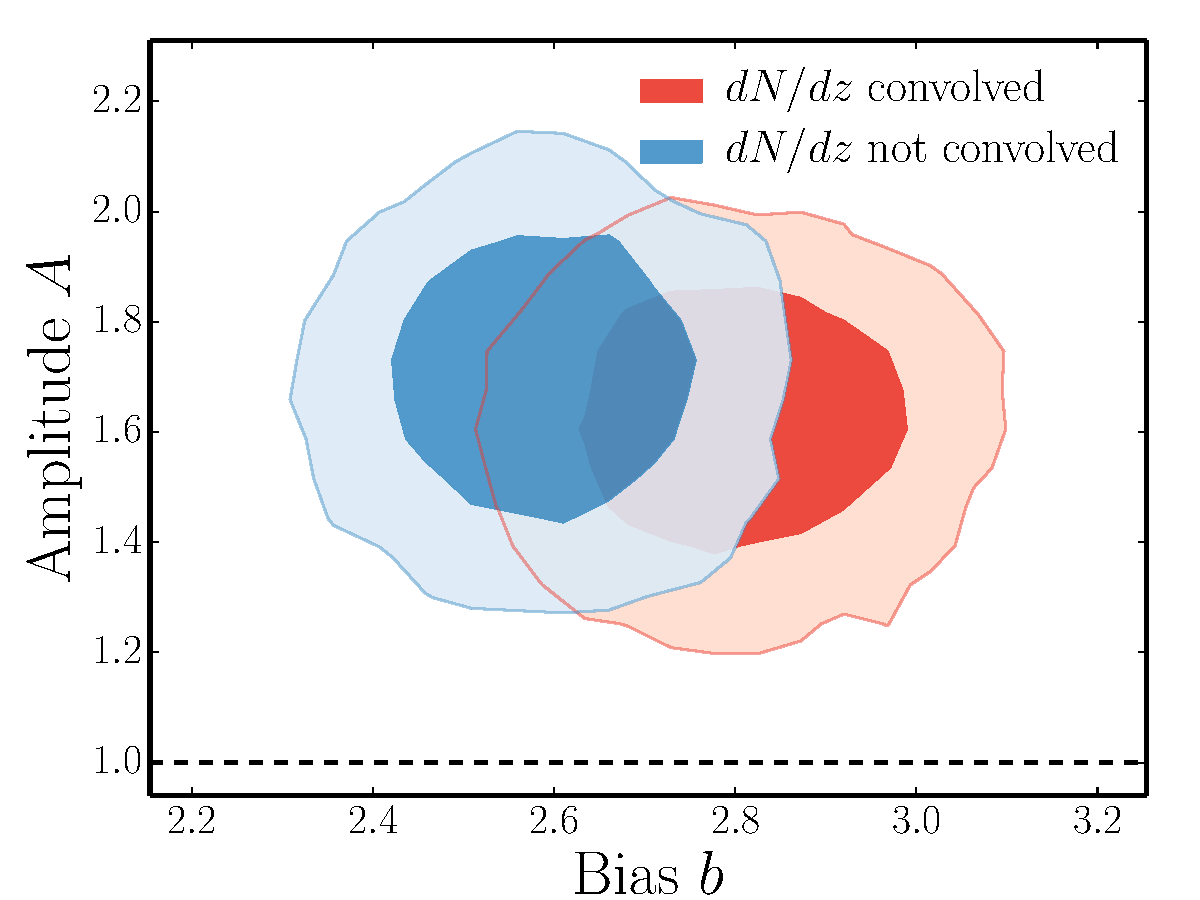
\includegraphics[width=0.7\textwidth]{Chapter3/Images/f19}
\caption{Posterior distributions for $A$ and $b$ obtained using the convolved (red contours) and the unconvolved $dN/dz$  (blue contours).  \label{fig:kg_gg_un_convolved_pdf}}
\end{figure}

\section{Conclusions}
\label{sec:conclusionsxc1}
We have presented the first measurement of the correlation between the lensing potential derived from the \emph{Planck} data and a high-$z$ ($z\ge 1.5$) galaxy catalog from the \emph{Herschel}-ATLAS survey, the highest redshift sample for which the correlation between \emph{Planck} \gls{CMB} lensing and tracers of large-scale structure has been investigated so far.
We have shown that the expected signal is remarkably strong, in spite of the small area covered by the H-ATLAS survey (about 1.3\% of the sky), suggesting that cross-correlation measurements between \gls{CMB} lensing maps and galaxy surveys can provide powerful constraints on the evolution of density fluctuations, on the nature of the \gls{DE}, and on properties of tracers of the matter distribution, provided that a good control of systematic errors  for both data sets can be achieved.

The null hypothesis (no correlation) was rejected with a significance of about $20\,\sigma$ and the significance of the detection of the theoretically expected cross-correlation signal was found to be $10\,\sigma$. The reliability of this result was confirmed by several null tests. A joint analysis of the cross-spectrum and of the autospectrum of the galaxy density contrast yielded a galaxy bias parameter of $b=2.80^{+0.12}_{-0.11}$, consistent with earlier estimates for H-ATLAS galaxies at similar redshifts. On the other hand, the amplitude of the cross-correlation was found to be a factor $1.62 \pm 0.16$ higher than expected from the standard model.

We have investigated possible reasons for the excess amplitude. Some of them, such as the redshift dependence of the bias parameter or the contamination by the Sunyaev-Zel'dovich effect, were found to be negligible. Others, such as the magnification bias due to weak gravitational lensing or errors in the photometrically estimated redshifts, can contribute significantly to the observed excess but cannot fully account for it. A possible culprit is some residual contamination of convergence maps by unresolved infrared sources \citep{Osborne2014,VanEngelen2014}, adding a substantial contribution to the measured correlation between the lensing convergence and the H-ATLAS high-$z$ sources, which are unresolved by \emph{Planck}. However, a detailed calculation of this effect is complicated and beyond the scope of the present chapter.

We have also investigated the possibility that the tension between the observed and the expected cross-correlation amplitude was overrated because the noise level of the convergence maps in the regions used for the cross correlation is above typical values. This turned out to be the case in the three GAMA fields, but the effect on the combination of fields was found to be marginal.

An exquisite mapping of the \gls{CMB} lensing pattern is one of the major goals of operating and planned \gls{CMB} probes because of its relevance in studying cosmological structure formation and the properties of the dark energy. Forthcoming data releases by \textit{Planck}\footnote{The \gls{CMB} lensing map from 2015 \textit{Planck} release will be used in the next chapter, while the definitive one, within the last data release expected for late 2016 could not be included in the present analysis.} as well as future \gls{CMB} lensing measurements from suborbital probes will be most relevant to further address the results presented here and improve the constraining power of these studies, both in a cosmological and astrophysical context.

